\chapter{视觉处理的构建本质} \label{chap:chap21}

我们对于视觉已经非常熟悉,以至于需要一次想象力的飞跃才能意识到还有问题需要解决。
但是考虑一下。
我们的眼睛接收到的是微小的、扭曲的、倒立的图像,而我们看到的却是周围空间中的独立实体。
我们从视网膜上的刺激模式中感知到了一个充满物体的世界,这简直就是一个奇迹。

\begin{flushright}
	———— \textit{理查德$\cdot$格里高利}, 《视觉心理学》, 1966 \hfill
\end{flushright}



我们对世界的大部分印象和我们对它的记忆都是基于视觉的。
然而,视觉背后的机制一点也不明显。
我们如何感知形状和运动?
我们如何区分颜色?
在复杂的视觉环境中识别物体是一项非凡的计算成就,人工视觉系统尚未复制。
视觉不仅用于识别物体,还用于指导我们的动作,这些独立的功能至少由两条并行且相互作用的通路调节。


视觉系统中并行通路的存在提出了认知的核心问题之一,即绑定问题:
不同类型的信息如何通过离散通路汇集到一个连贯的视觉图像中?



\section{视觉感知是一个构造的过程}

视觉经常被错误地比作照相机的操作。
照相机简单地逐点再现视野的一个平面中的光强度。
相比之下,视觉系统做了一些根本不同的事情。
它解释场景并将其解析为不同的组件,将前景与背景分开。
在某些任务中,视觉系统不如相机准确,例如量化亮度的绝对水平或识别光谱颜色。
然而,它擅长识别正在奔跑的动物、超速行驶的汽车等任务,无论是在明亮的阳光下还是在黄昏,在开阔的田野中还是被树木(或其他汽车)部分遮挡。
它如此迅速地让观众做出反应,并在必要时逃脱。


一个潜在的统一见解可以调和视觉系统掌握大局的非凡能力及其对输入细节的不准确性,即视觉是一个生物过程,它是随着我们的生态需求而进化的。
这种洞察力有助于解释为什么视觉系统在提取有用信息(例如独立于照明条件的对象的身份)方面如此有效,同时对环境光的确切性质等方面不太重视。
此外,视觉使用先前学习的关于世界结构的规则来做到这一点。
在进化过程中,其中一些规则似乎已经连接到我们的神经回路中。
其他人则更具可塑性,可以帮助大脑根据个人过去的经验猜测呈现在眼前的场景。
这种复杂的、有目的的处理发生在视觉系统的各个层面。 
它甚至从视网膜开始,视网膜专门用于挑选物体边界,而不是创建均匀表面的逐点表示。


视觉感知的这种建设性性质直到最近才得到充分认识。
早期关于感官知觉的思考深受英国经验主义哲学家的影响,尤其是\textit{约翰$\cdot$洛克}、\textit{大卫$\cdot$休谟}和\textit{乔治$\cdot$伯克利},他们认为知觉是一个原子过程,在这个过程中,简单的感官元素,如颜色、形状和亮度,被组合在一起 以一种添加的方式,逐个组件。
现代观点认为知觉是一种积极的创造性过程,不仅仅涉及提供给视网膜的信息,其根源在于伊曼纽尔康德的哲学,并在 20 世纪初由德国心理学家\textit{马克斯$\cdot$韦特海默},\textit{库尔特$\cdot$考夫卡}详细发展 和\textit{沃尔夫冈$\cdot$苛勒},他创立了格式塔心理学学院。


德语术语格式塔表示配置或形式。
格式塔心理学家的中心思想是,我们对刺激的看法(我们对任何视觉目标的感知解释)不仅取决于刺激的特性,还取决于刺激的背景,取决于视野中的其他特征。
格式塔心理学家认为,视觉系统根据系统固有的计算规则处理关于物体的形状、颜色、距离和运动的感官信息。
大脑有一种看待世界的方式,即部分源自经验、部分源自内置神经线路的一系列期望。


\textit{马克斯$\cdot$韦特海默}写道:“在某些实体中,整体的行为既不能源自其单个元素,也不能源自这些元素组合在一起的方式;
恰恰相反:任何部分的属性都由整体的内在结构法则决定。” 
在 20 世纪早期,格式塔心理学家制定了感知法则,这些法则决定了我们如何对视觉场景中的元素进行分组,包括相似性、接近性和连续性。


由于视觉系统倾向于强加一种模式,我们看到一个统一的六乘六点阵列作为行或列。
如果每行中的点相似,我们更有可能看到交替行的模式(图~\ref{fig:21_1}A)。
如果每列中的点比行中的点靠得更近,我们更倾向于看到列的模式(图~\ref{fig:21_1}B)。
良好连续性原则是将线元素连接成统一形状的重要基础(图~\ref{fig:21_1}C)。
它也出现在轮廓显著现象中,平滑的轮廓往往会从复杂的背景中弹出(图~\ref{fig:21_1}D)。
我们倾向于挑选出的格式塔特征也是表征自然场景中物体的特征。
对自然场景的统计研究表明,目标边界可能包含非常接近的视觉元素,在交叉点上是连续的,或者形成平滑的轮廓。
很容易推测自然场景中物体的形式特征对我们的视觉系统产生了进化压力,以发展出使我们对这些特征敏感的神经回路。


\begin{figure}[htbp]
	\centering
	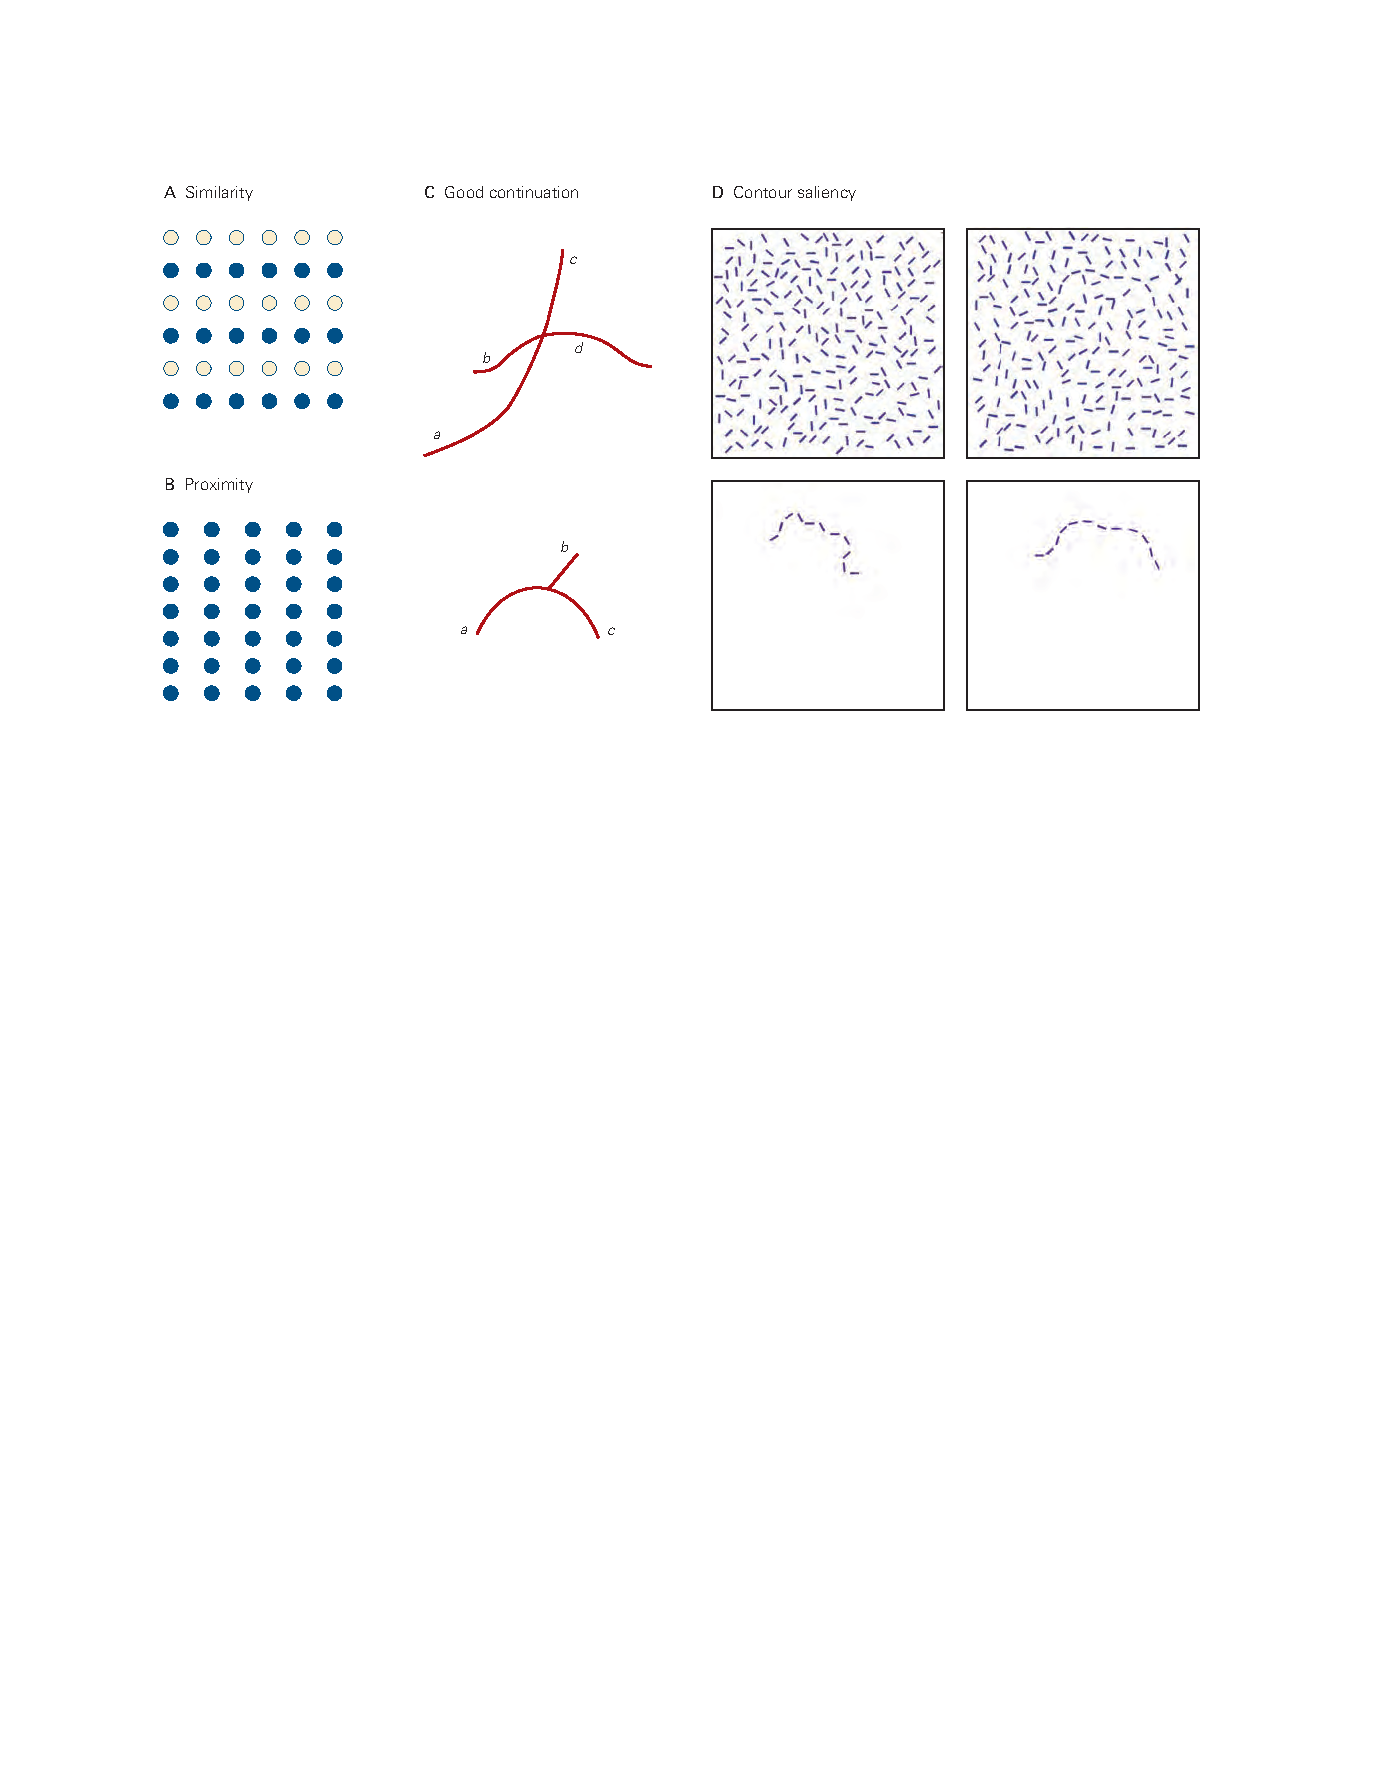
\includegraphics[width=1.0\linewidth]{chap21/fig_21_1}
	\caption{视觉感知的组织规则。
		为了将视觉场景的元素连接成统一的感知,视觉系统依赖于组织规则,如相似性、接近性和良好的连续性。
		\textbf{A.} 因为交替行中的点具有相同的颜色,所以整体图案是蓝色和白色行。
		\textbf{B.} 列中的点比行中的点靠得更近,导致列的感知。
		\textbf{C.} 当线段共线时,它们在感知上是相连的。
		在顶部的一组线中,人们更有可能将线段 a 视为属于 c 而不是 d。
		在底部集合中,a 和 c 在感知上是相关的,因为它们保持相同的曲率,而 a 和 b 似乎是不连续的。
		\textbf{D.} 良好连续性原则也见于轮廓显著性。
		在右侧,线条元素的平滑轮廓从背景中弹出,而左侧的锯齿状轮廓消失在背景中\cite{field1993contour}。}
	\label{fig:21_1}
\end{figure}


分离视觉场景中的人物和背景是物体识别的重要步骤。
在不同的时刻,视野中的相同元素可以组织成一个可识别的图形或作为其他图形的背景的一部分(图~\ref{fig:21_2})。
这种分割过程不仅依赖于某些几何原理,还依赖于注意力和期望等认知影响。
因此,启动刺激或物体形状的内部表示可以促进视觉元素的关联,形成统一的感知(图\ref{fig:21_3})。
这种内部表示可以采用许多不同的形式,反映神经编码的广泛时间尺度和机制。
它可能包括对形状或决定有选择性的瞬态回响尖峰活动,持续几分之一秒,或在任务的特定上下文或预期形状期间选择性调制突触权重,或可能包含长期记忆的回路变化。


\begin{figure}[htbp]
	\centering
	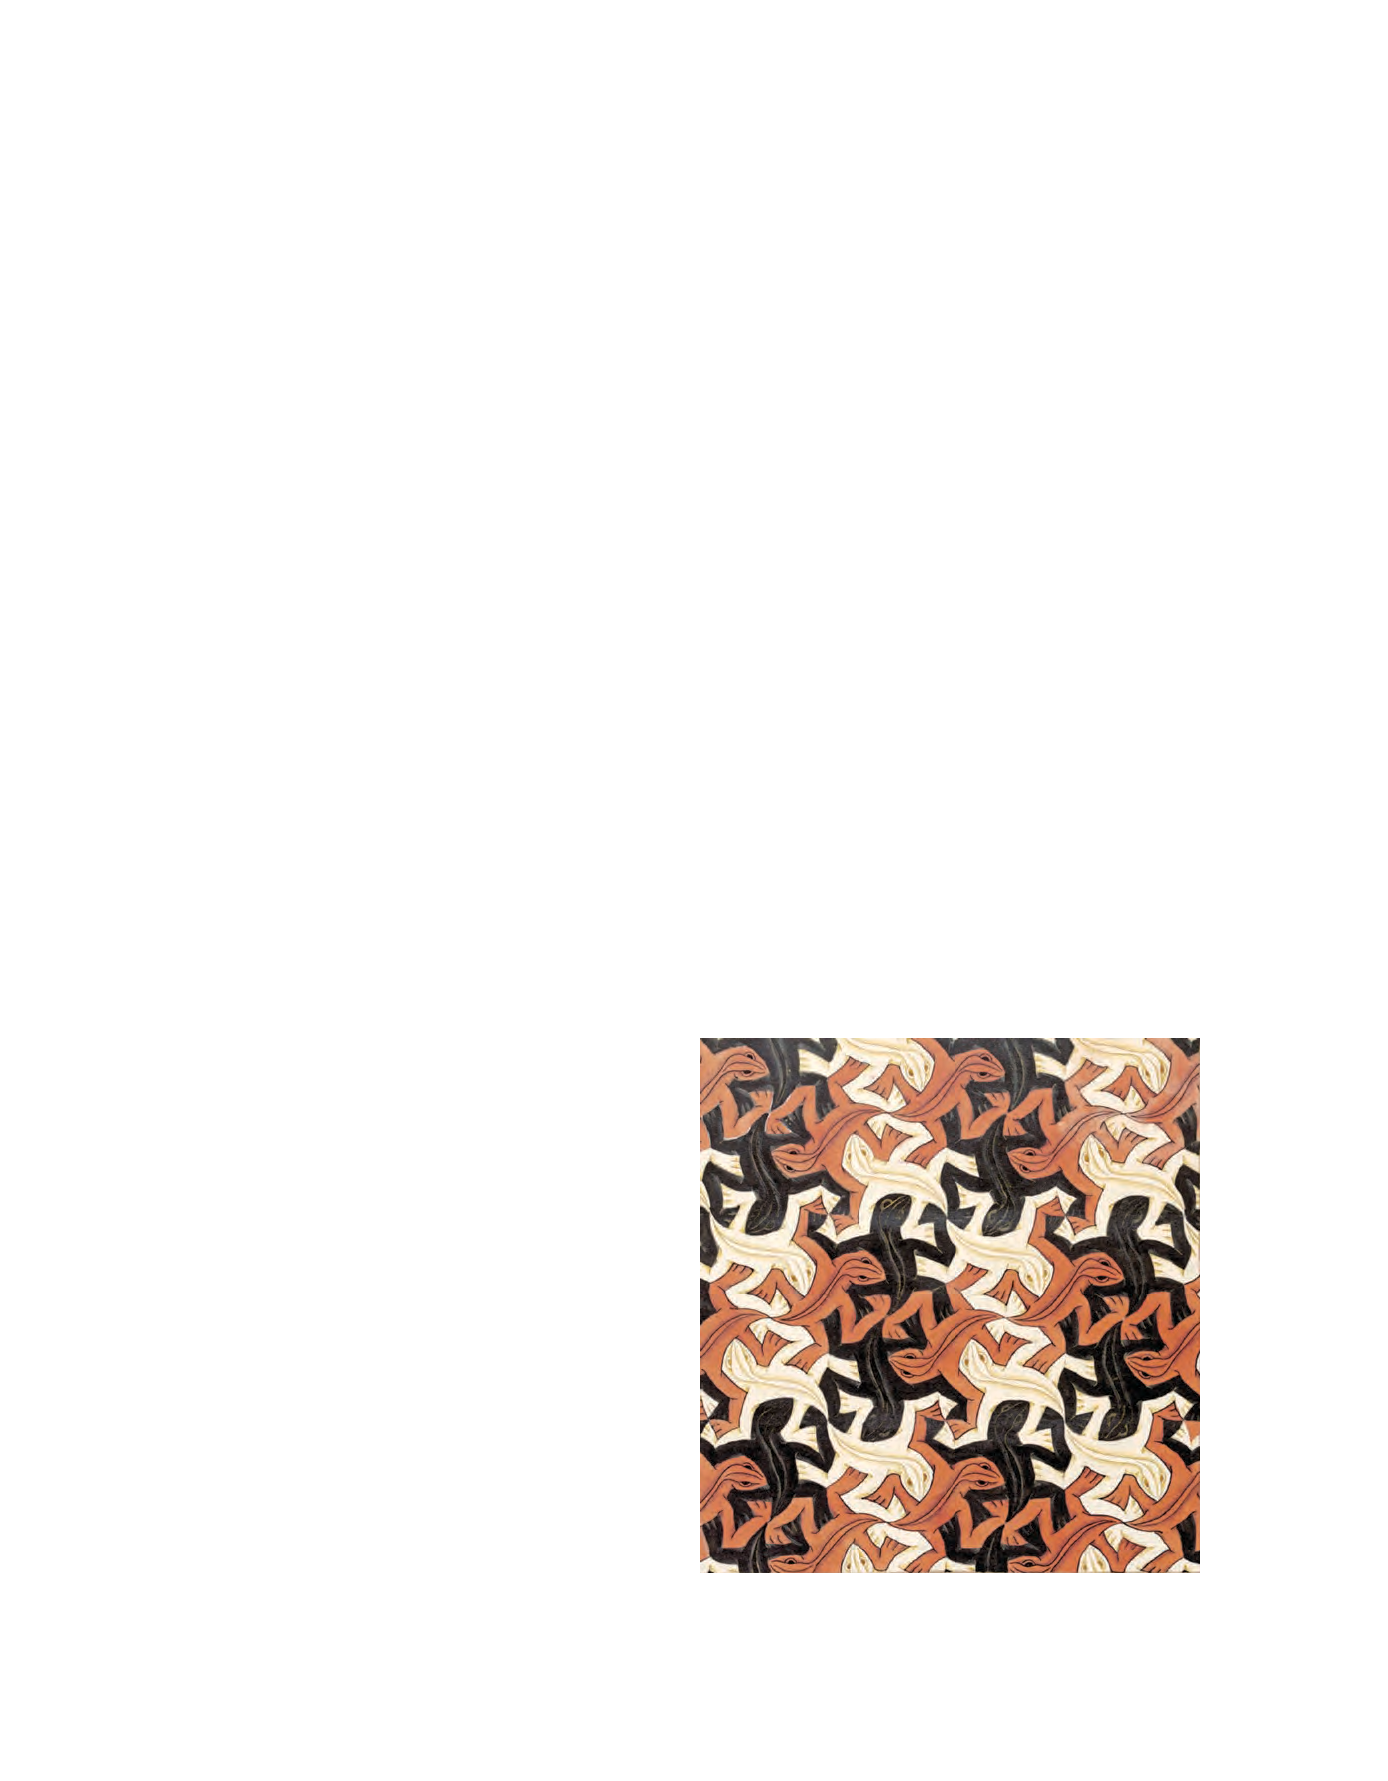
\includegraphics[width=0.5\linewidth]{chap21/fig_21_2}
	\caption{目标识别取决于将场景分割成前景和背景。
		在此图像中识别白色蝾螈取决于大脑“定位”前景中的白色蝾螈和背景中的棕色和黑色蝾螈。
		该图像还说明了较高影响在分割中的作用:
		人们可以有意识地选择三种颜色中的任何一种作为前景。}
	\label{fig:21_2}
\end{figure}


\begin{figure}[htbp]
	\centering
	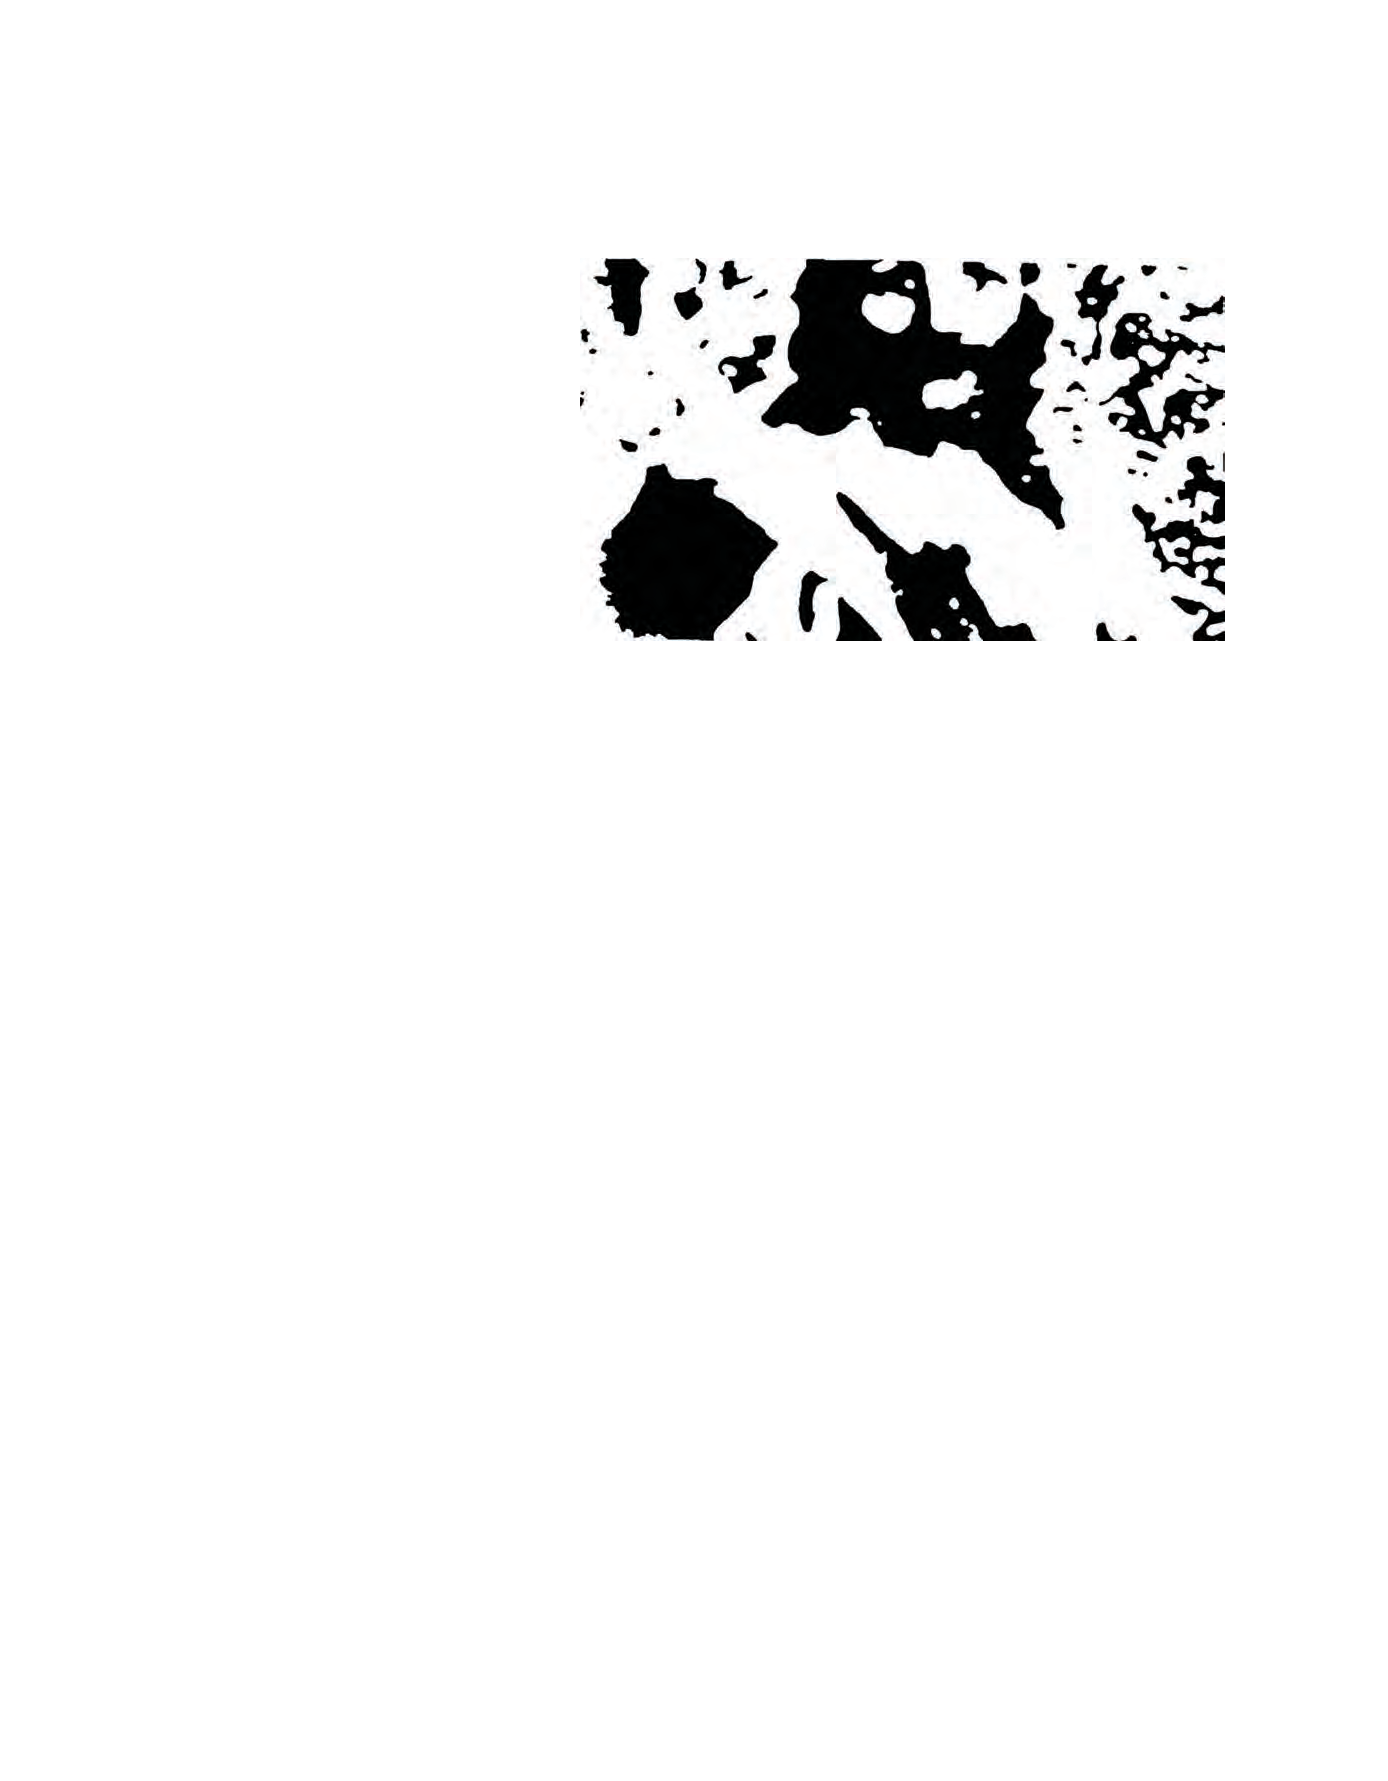
\includegraphics[width=0.7\linewidth]{chap21/fig_21_3}
	\caption{期望和感知任务在所见事物中起着至关重要的作用。
		如果没有附加信息,很难将此图中的黑色和白色色块分成前景和背景。
		在查看图~\ref{fig:21_3_1}~上的启动图像后,该图立即变得可识别。
		在此示例中,形状的高阶表示指导表面分割的低阶过程。}
	\label{fig:21_3}
\end{figure}


大脑在三个级别分析视觉场景:低层、中层和高层(图~\ref{fig:21_4} )。
在我们下一章(第~\ref{chap:chap22}~章)考虑的最低层,视觉属性如局部对比度、方向、颜色和运动被区分。
中层涉及场景布局和表面属性的分析,将视觉图像解析为表面和全局轮廓,以及区分前景和背景(第~\ref{chap:chap23}~章)。
最高层涉及目标识别(第~\ref{chap:chap24}~章)。
一旦场景被大脑解析并识别出物体,物体就可以与形状记忆及其相关含义相匹配。
视觉在引导身体运动,尤其是手部运动方面也具有重要作用(第~\ref{chap:chap25}~章)。


\begin{figure}[htbp]
	\centering
	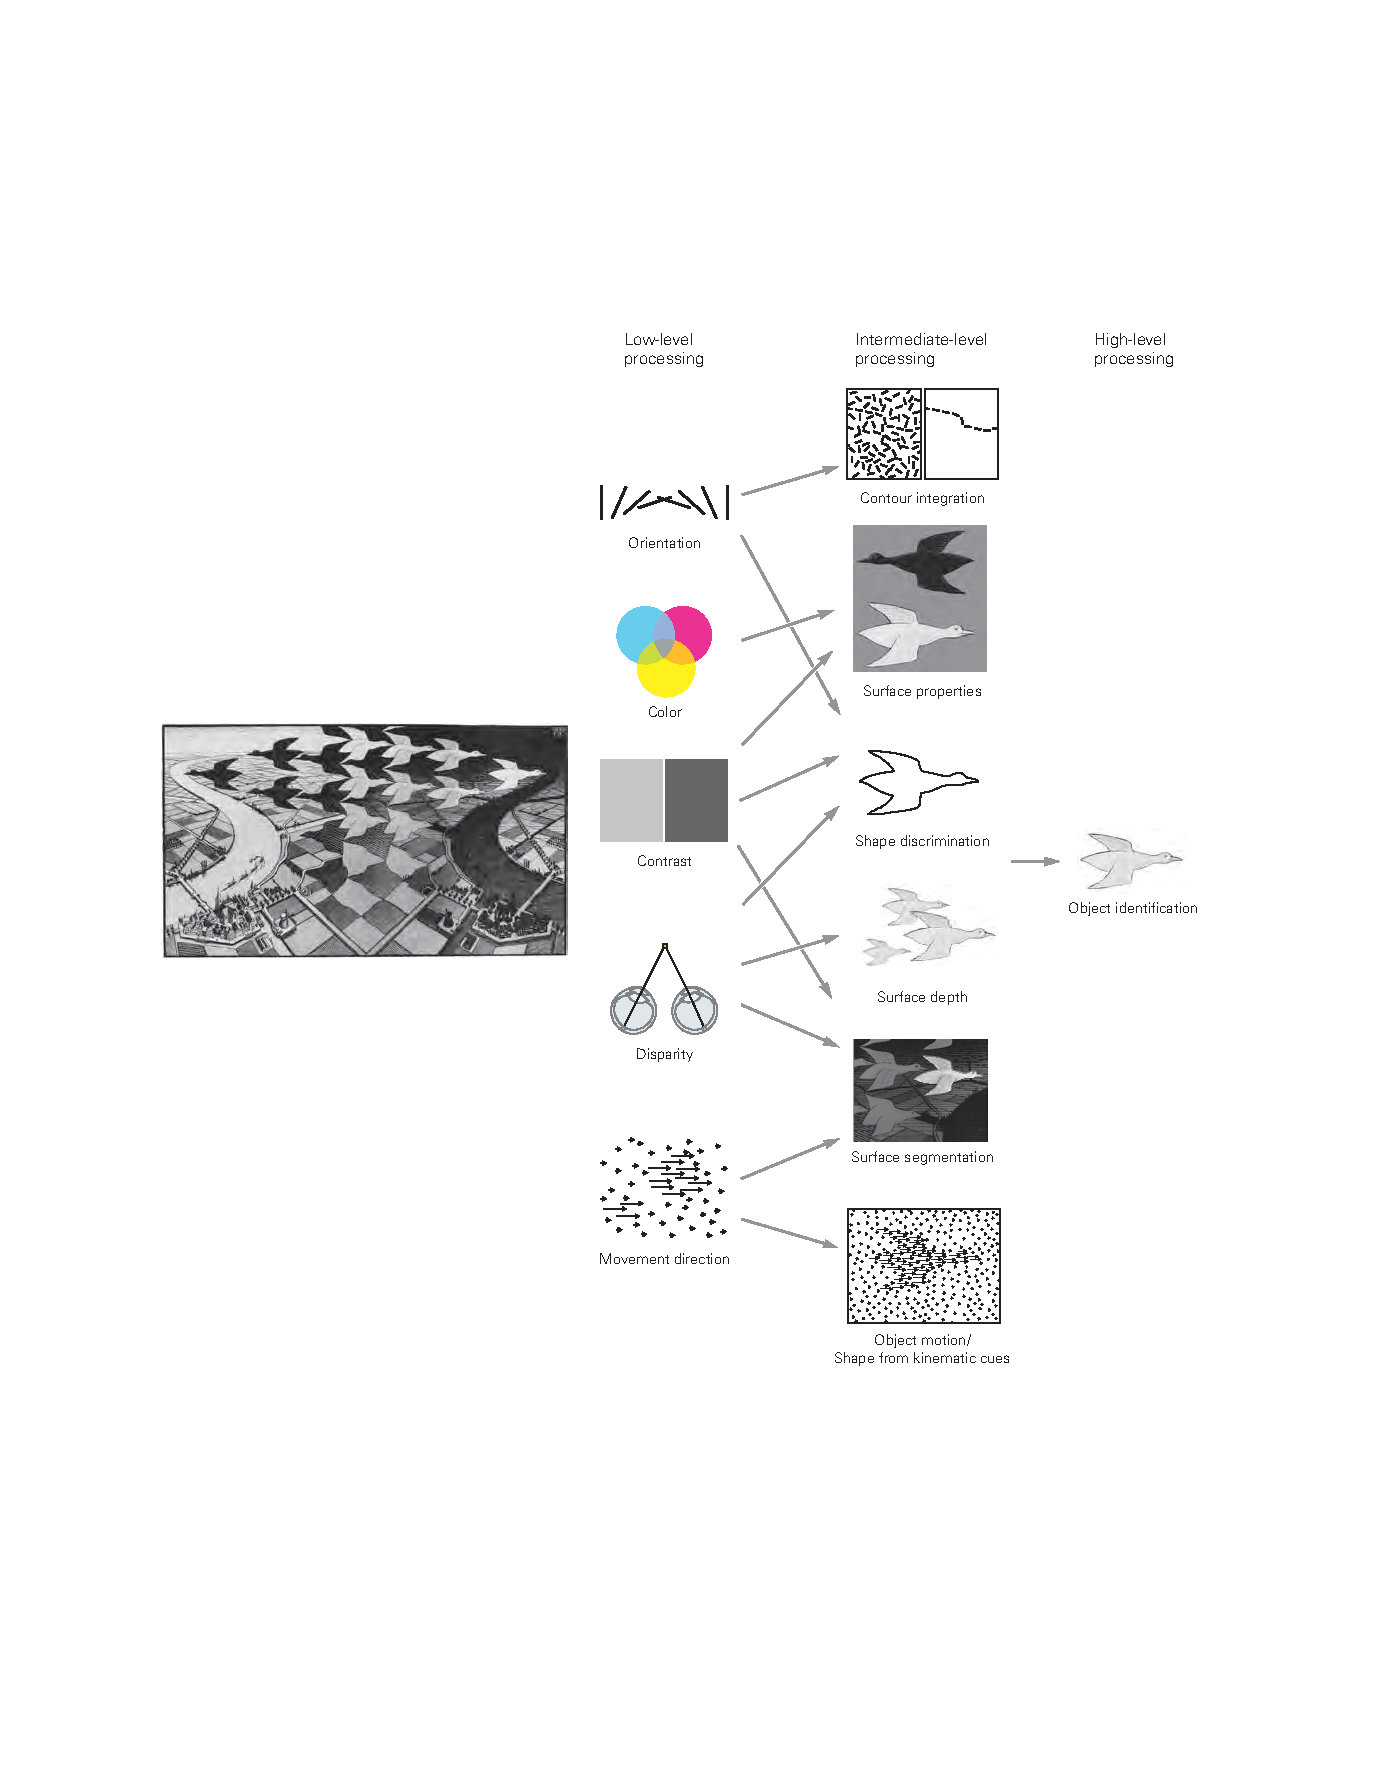
\includegraphics[width=1.0\linewidth]{chap21/fig_21_4}
	\caption{视觉场景在三个层次上进行分析。
		分析视觉环境的简单属性(低层处理),然后使用这些低级特征来解析视觉场景(中层处理):
		局部视觉特征被组装成表面,物体与背景分离(表面分割),局部方向被整合到全局轮廓中(轮廓整合),表面形状从阴影和运动学线索中识别。
		最后,表面和轮廓用于识别目标(高层处理)。}
	\label{fig:21_4}
\end{figure}


在视觉中,就像在其他认知操作中一样,各种特征(运动、深度、形式和颜色)一起出现在一个统一的知觉中。
这种统一不是通过一个分层的神经系统实现的,而是通过大脑中的多个区域实现的,这些区域由平行但相互作用的神经通路提供。
由于分布式处理是视觉神经生物学中的主要组织原则之一,因此必须掌握视觉系统的解剖通路,才能在后面的章节中充分理解视觉处理的生理描述。


在本章中,我们为理解视觉通路的神经回路和组织原则奠定了基础。
这些原则应用非常广泛,不仅与大脑中与视觉有关的多个区域相关,而且与大脑处理其他类型的感觉信息有关。



\section{视觉处理由膝纹通路调制}

大脑对视觉场景的分析始于两个视网膜,它们使用并行处理策略转换视觉输入(第~\ref{chap:chap22}~章)。
这种重要的神经计算策略被用于视觉通路的所有阶段以及其他感觉区域。
落在单个光感受器(视杆细胞和视锥细胞)上的像素状视觉输入由视网膜回路分析以提取大约 20 种局部特征,例如暗与光、红与绿、蓝与黄的局部对比。
这些特征由不同群体的专门神经回路计算,形成独立的处理模块,分别覆盖视野。
因此,视野中的每个点都在多个通道中处理,这些通道同时并行地提取视觉输入的不同方面。
然后这些平行流沿着视网膜神经节细胞的轴突发出,视网膜的投射神经元,形成视神经。


从眼睛开始,视神经延伸到中线交叉点,即视交叉。
在交叉之外,来自每个颞侧视网膜的纤维沿着同侧视束行进到同侧半球;
来自鼻侧视网膜的纤维沿着对侧视束穿过对侧半球(图~\ref{fig:21_5})。
因为一只眼睛的颞侧半视网膜与另一只眼睛的鼻侧半视网膜看到相同的一半视野(半视野),所以交叉处纤维的部分交叉确保了关于每个半视野的所有信息都在视觉皮层中对侧半球处理。 。
通路的布局也构成了有用诊断信息的基础。
由于该视觉通路的特殊解剖结构,沿通路不同点的病变导致具有不同几何形状的视觉缺陷(图~\ref{fig:21_5}),可以通过临床检查可靠地区分。
缺陷可能完全是单眼的;
如果出现在双眼中,它可能会影响双眼视野中的非对应或对应部分;
它可能仅限于上部或下部视野,也可能延伸到两者。
因此,缺陷的形状可以提供有关潜在神经损伤或闭塞的类型和位置的有价值线索(范围从视神经变性,例如由于多发性硬化症、肿瘤、中风或身体创伤)。


\begin{figure}[htbp]
	\centering
	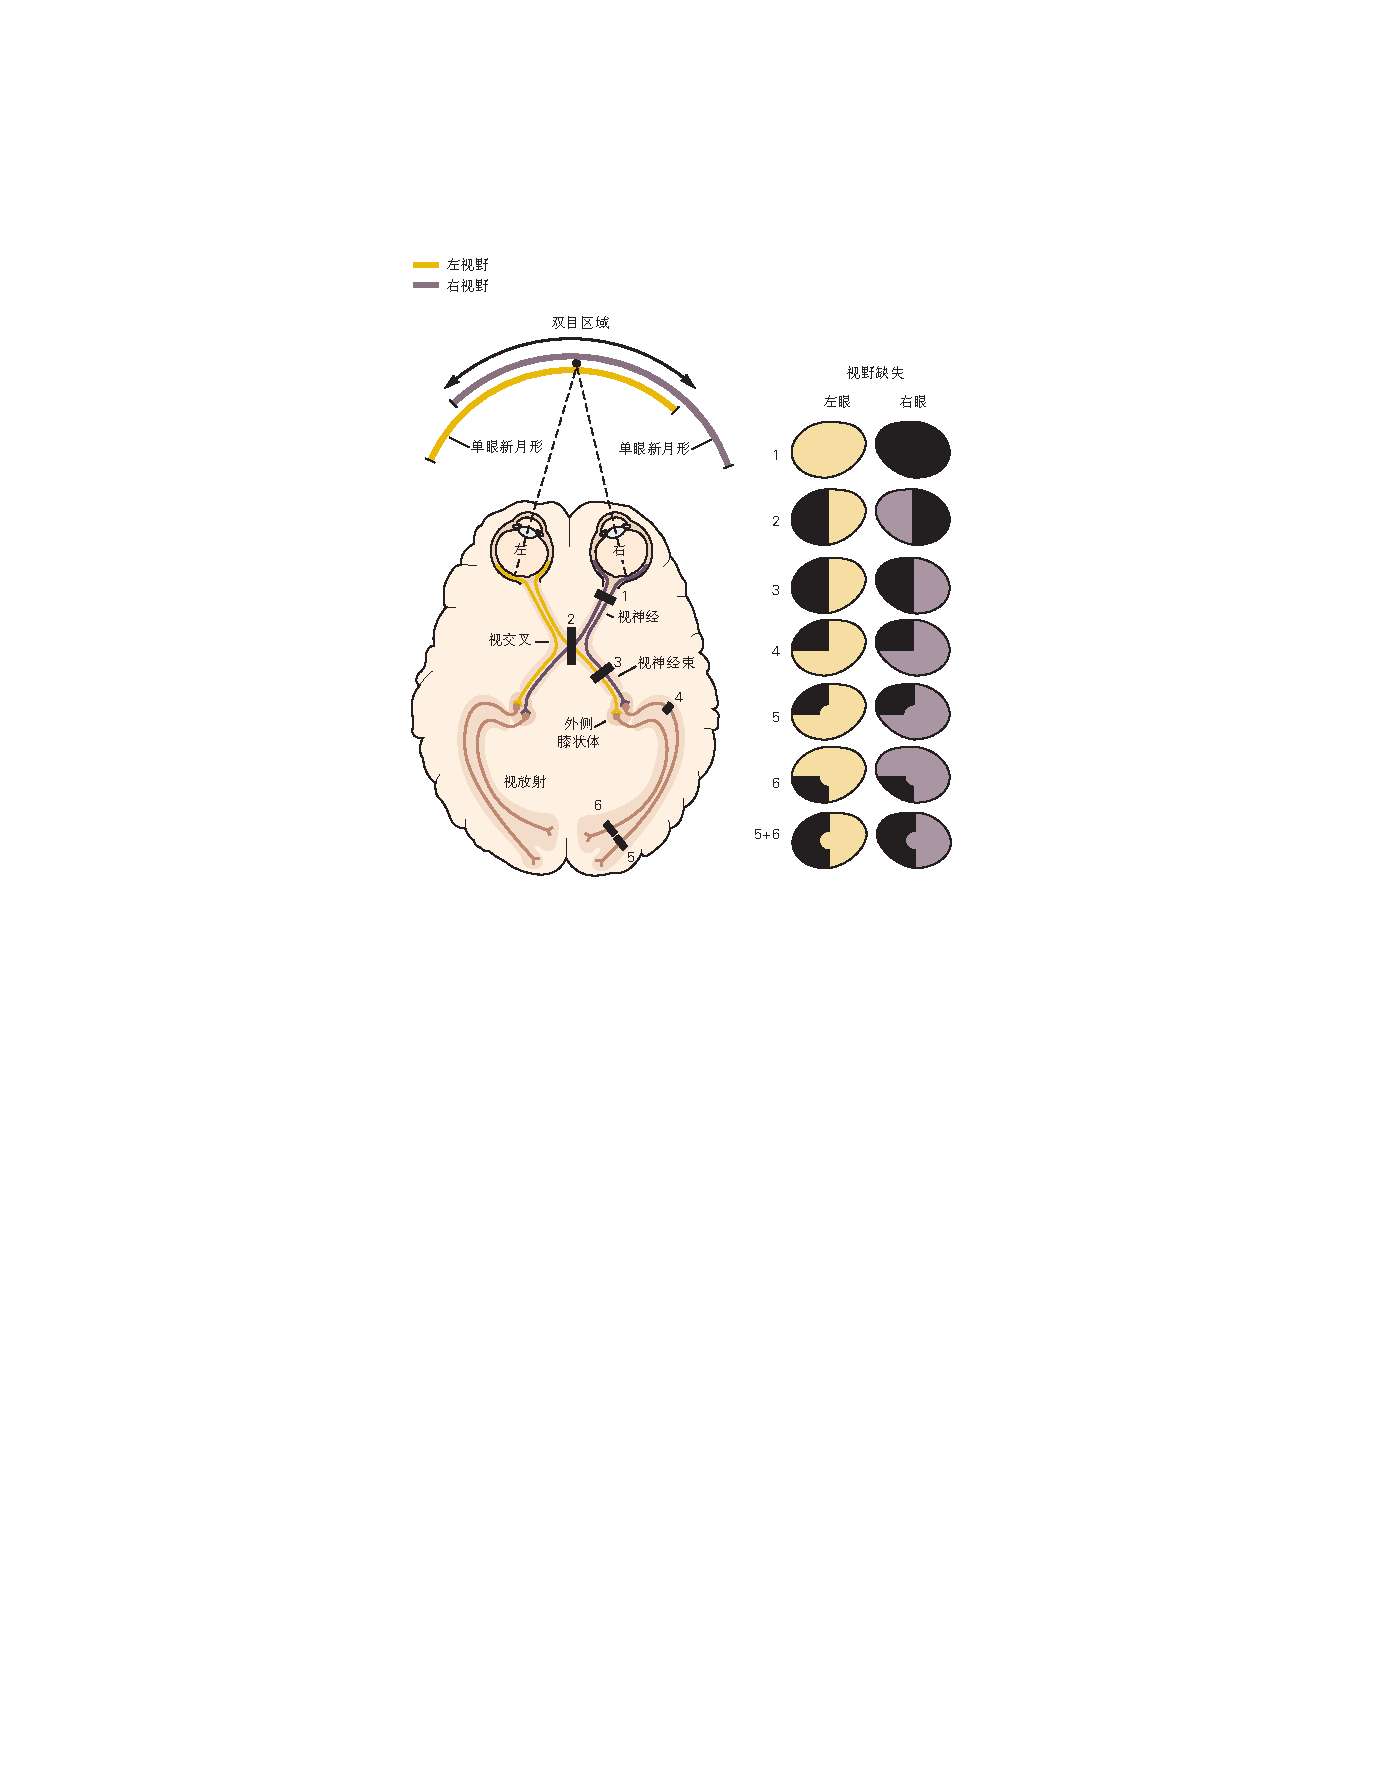
\includegraphics[width=0.65\linewidth]{chap21/fig_21_5}
	\caption{沿视觉通路的视野表示。
		每只眼睛都能看到大部分视野,除了被称为单眼新月的一部分周边视野。
		视网膜神经元(神经节细胞)的轴突将信息从每个视觉半场沿视神经传递到视交叉,鼻侧半视网膜的纤维在这里交叉到对侧半球。
		来自颞侧视网膜的纤维留在同一侧,连接来自对侧眼的鼻侧视网膜的纤维形成视束。
		视束携带来自双眼的对侧视觉半场的信息,并投射到外侧膝状体核中。
		这个细胞核中的细胞将它们的轴突沿着视辐射发送到初级视觉皮层。
		沿视觉通路的病变会产生特定的视野缺损,如右图所示:
		1. 视神经病变会导致一只眼睛完全丧失视力。
		2. 视交叉损伤导致每个视觉半场的颞半部视力丧失(双颞侧偏盲)。
		3. 视束损伤导致另一半半视野视力丧失(对侧偏盲)。
		4. 弯曲进入颞叶(\textit{梅耶环束})的视辐射纤维损伤导致双眼对侧半视野上象限视力丧失(对侧上象限性失明)。
		5, 6. 视觉皮层的部分损伤导致对侧视觉半场的部分缺陷。
		例如,距状沟(5)上岸的病变会导致下象限的部分缺陷,而下岸(6)的病变会导致上象限的部分缺陷。 由于中央凹的表现范围和半球垂直子午线的重复表现,视野的中心区域往往不受皮层病变的影响。}
	\label{fig:21_5}
\end{figure}


\begin{figure}[htbp]
	\centering
	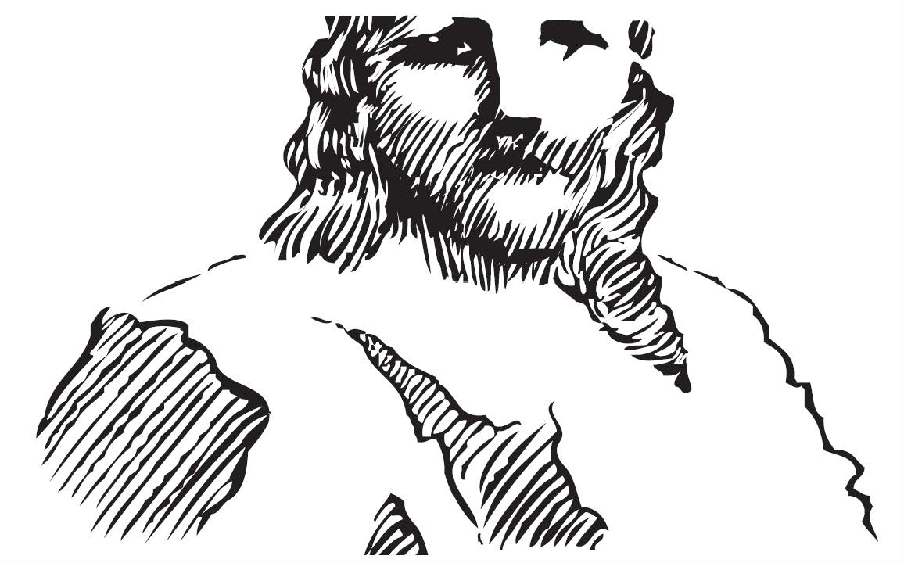
\includegraphics[width=0.7\linewidth]{chap21/fig_21_3_1}
	\caption{图~\ref{fig:21_3}~的启动图片。}
	\label{fig:21_3_1}
\end{figure}


在视交叉之外,来自鼻侧和颞侧半视网膜的轴突携带来自一侧半视野的输入,加入视束,延伸至丘脑的外侧膝状体核。
灵长类动物的\textit{外侧膝状体}由六个主要层组成:四个小细胞层和两个大细胞层,每个层都与薄但致密的插层或粒状层配对(见图~\ref{fig:21_14})。
术语“粒状”指的是这些层中的细胞体相对于大细胞或小细胞层的细胞体要小得多。
视网膜中建立的平行通道通过\textit{外侧膝状体}在解剖学上保持隔离。
细小细胞层从小型视网膜神经节细胞获得输入,这些细胞在灵长类动物视网膜中数量最多 (70\%),并携带红绿色对手信息(第~\ref{chap:chap22}~章)。
大细胞层从伞状神经节细胞(10\%)获得消色差对比信息。
\textit{粒状}层从小型和大型双层神经节细胞获得输入,携带蓝黄色信息,它们共同构成第三大群体最多的\textit{外侧膝状体}视网膜投射集(8\%)。
\textit{粒状}层也从许多其他数量上更小的视网膜神经节细胞类别获得输入。


每个膝状体层接收来自同侧或对侧眼的输入(参见图~\ref{fig:21_12} ),但被对齐以来自对侧半视野的匹配区域。
因此,它们形成了一组相互堆叠的一致地图。
然后丘脑神经元将视网膜信息传递到初级视觉皮层。
但是外侧膝状体不仅仅是一个转发器;
它接收到的视网膜信息可以通过与该大脑区域的抑制性连接以及来自视觉皮层的反馈受到注意力和唤醒的强烈调节。


\begin{figure}[htbp]
	\centering
	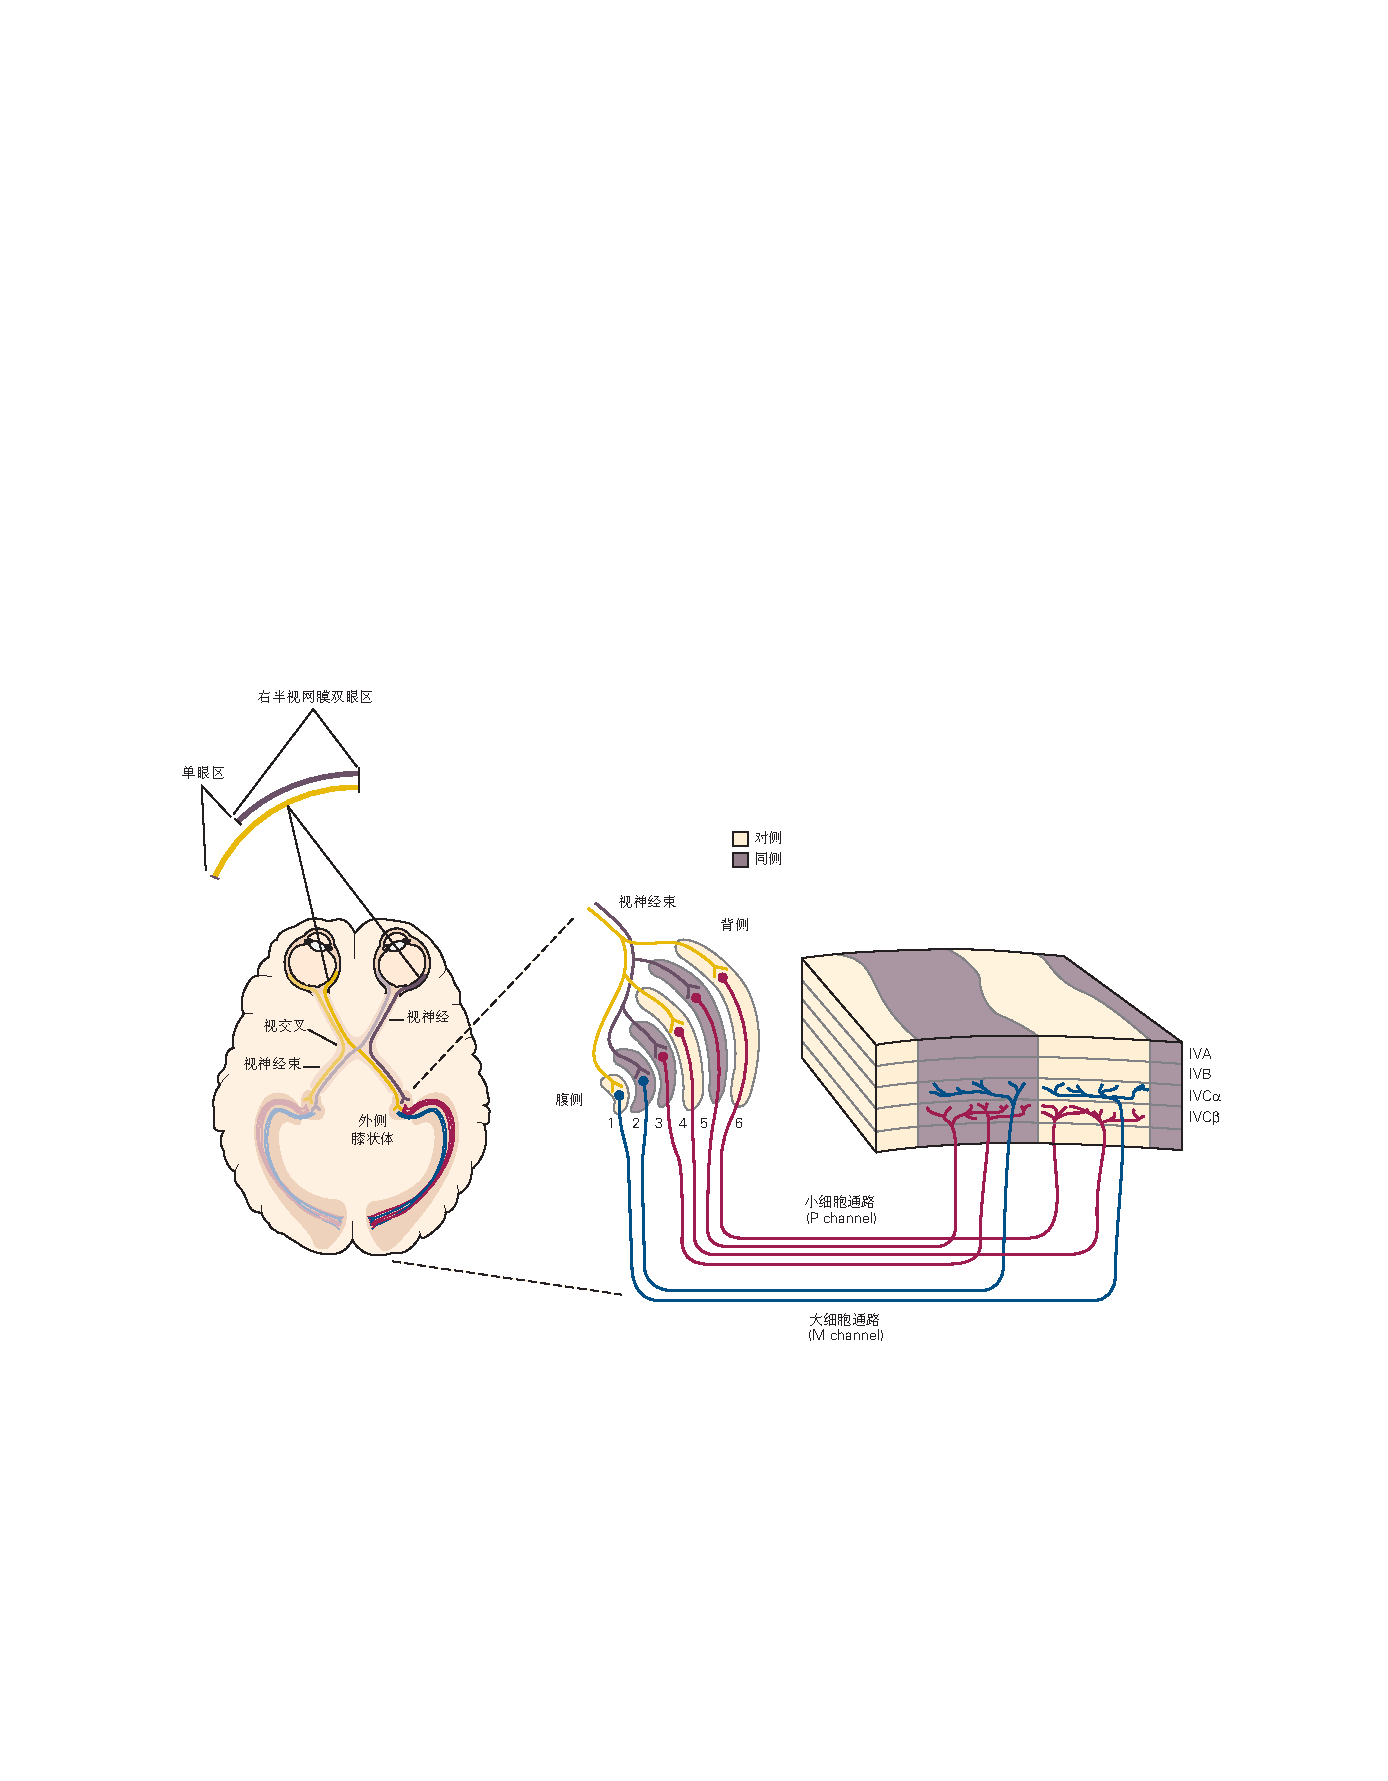
\includegraphics[width=1.0\linewidth]{chap21/fig_21_12}
	\caption{从外侧膝状体到视觉皮层的投射。
		每个半球的外侧膝状体核接收来自同侧眼的颞侧视网膜和对侧眼的鼻侧视网膜的输入。
		细胞核是一种分层结构,包括四个小细胞层(第 3 至 6 层)和两个大细胞层(第 1 层和第 2 层)。
		每个都与插入的\textit{粒状}层配对。
		(这些层在这里由分隔主要层的间隙表示。
		它们没有标记以避免混乱。
		参见图~\ref{fig:21_14}。)
		来自两只眼睛的输入终止于不同的膝状体层:
		对侧眼投射到层 1、4、 和 6,而同侧眼睛将输入发送到第 2、3 和 5 层。
		来自这些膝状体层的神经元然后投射到皮层的不同层。
		小细胞膝状体神经元投射到 IVC$\beta$ 层,大细胞神经元投射到 IVC$\alpha$ 层,而\textit{粒状}神经元投射到上皮层的“斑点”(见图~\ref{fig:21_14} 和~\ref{fig:21_15})。
		此外,来自外侧膝状体同侧和对侧层的传入神经被分离到交替的眼优势柱中。}
	\label{fig:21_12}
\end{figure}


主要视觉通路也称为膝纹通路(图~\ref{fig:21_6} A),因为它在到达初级视觉皮层的途中穿过外侧膝状体,也称为纹状皮层,因为富含髓磷脂的条纹贯穿其中。
第二条通路从视网膜延伸到中脑的前顶盖区域,神经元在此处调节控制进入眼睛的光量的瞳孔反射(图~\ref{fig:21_6}B)。
第三条通路从视网膜延伸到上丘,对控制眼球运动很重要。
该通路继续到脑干中的桥脑形成,然后到眼外运动核(图~\ref{fig:21_6}C)。


\begin{figure}[htbp]
	\centering
	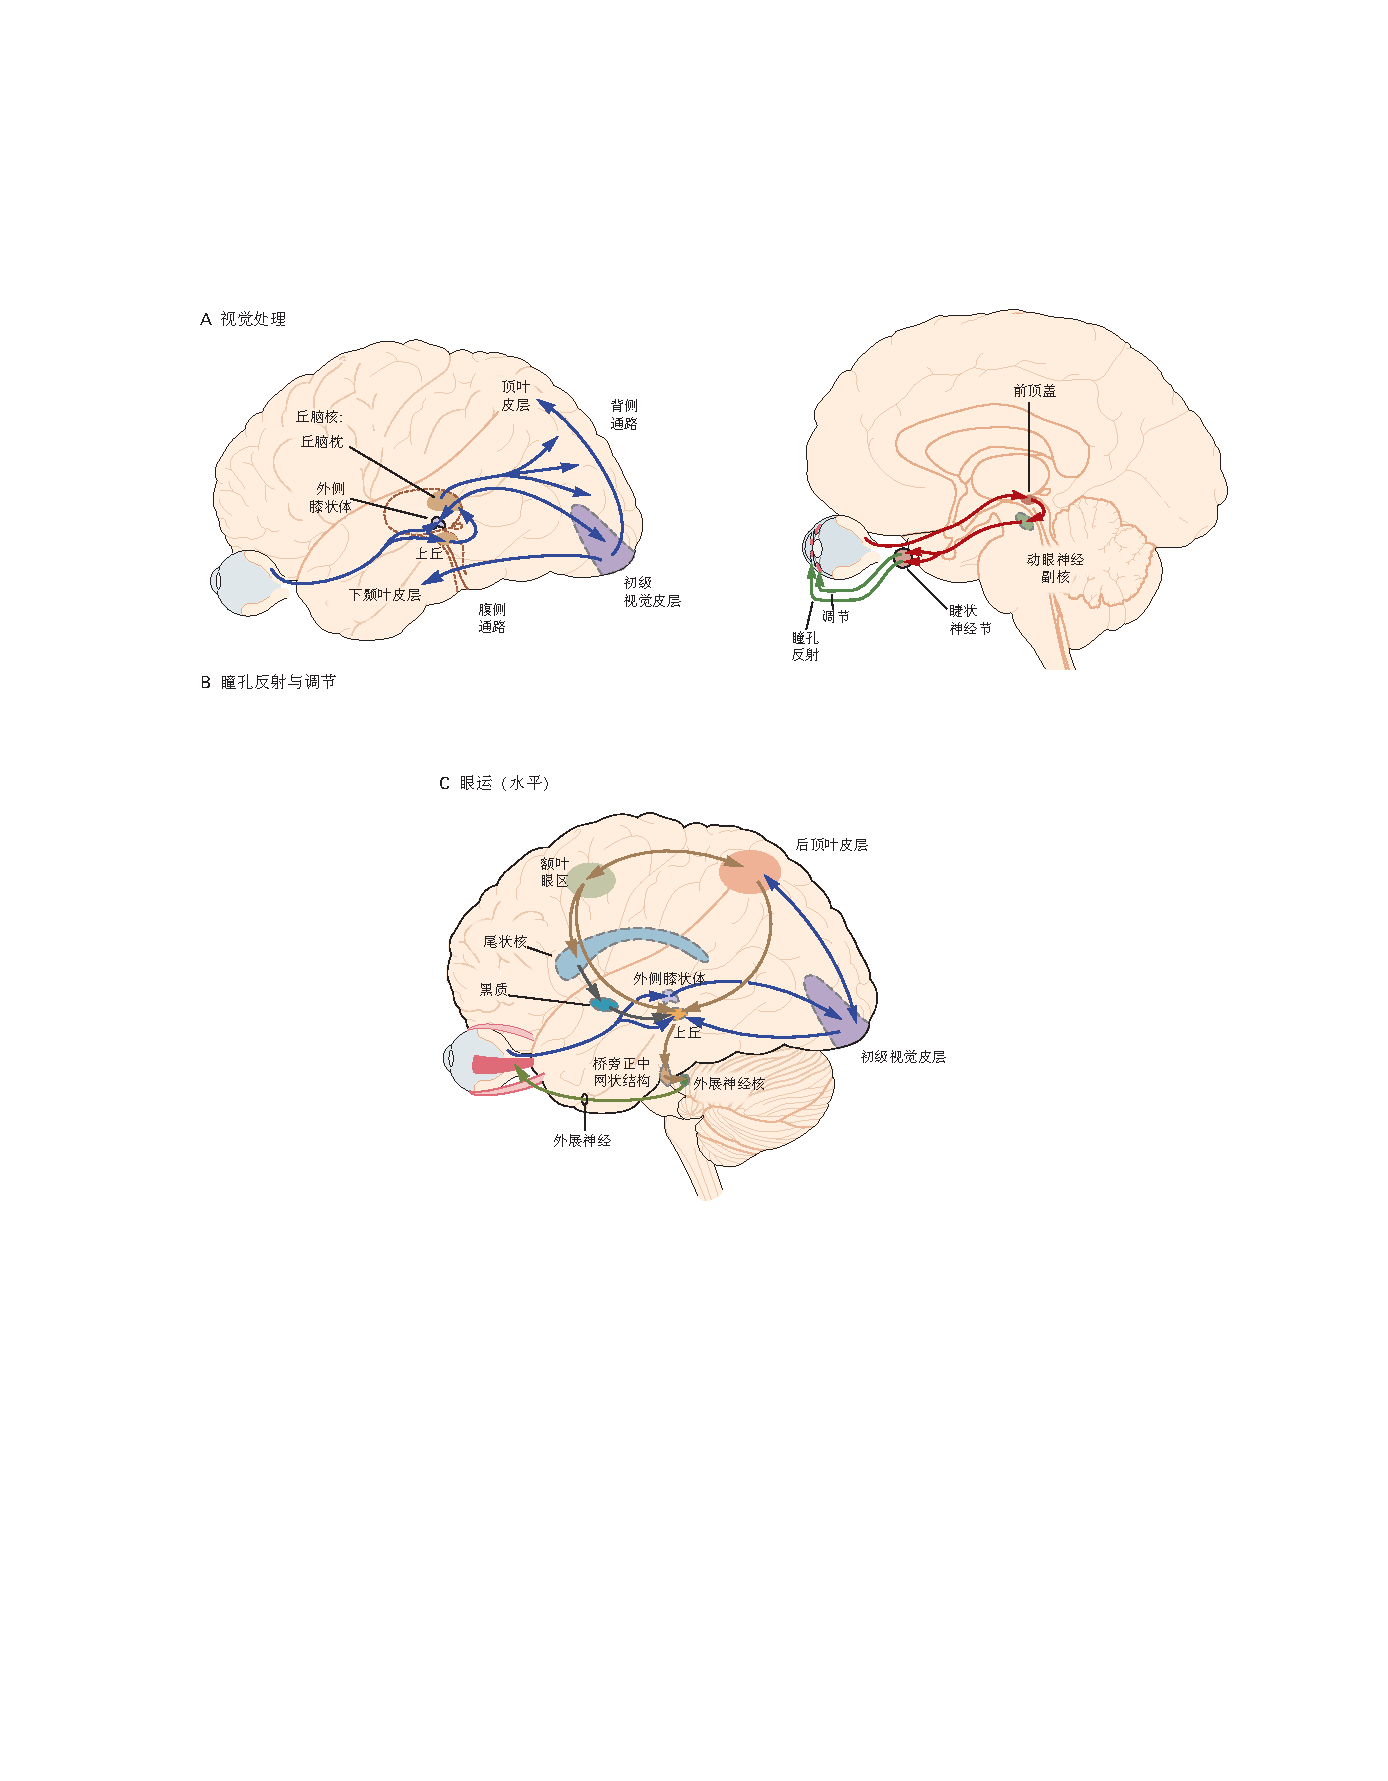
\includegraphics[width=1.0\linewidth]{chap21/fig_21_6}
	\caption{视觉处理、瞳孔反射和调节以及眼位控制的途径。
		\textbf{A.} 视觉处理。
		眼睛首先将信息发送到丘脑核团,包括外侧膝状体核和枕核,然后从那里发送到皮层区域。
		皮层投射从初级视觉皮层向前延伸到顶叶区域(与视觉引导运动有关的背侧通路)和颞叶区域(与物体识别有关的腹侧通路)。
		枕还充当皮层区域之间的中继以补充它们的直接连接。
		\textbf{B.} 瞳孔反射和调节。
		光信号通过中脑前顶盖传递到\textit{动眼神经副核}中的节前副交感神经元,并通过动眼神经的副交感神经流出到睫状神经节。
		节后神经元支配瞳孔括约肌的平滑肌,以及控制晶状体的肌肉。
		\textbf{C.} 眼球运动。
		来自视网膜的信息沿着视神经直接发送到\textit{上丘},并通过膝纹通路间接发送到投射回上丘的皮层区域(初级视觉皮层、后顶叶皮层和\textit{额叶视区})。
		丘投射到\textit{脑桥旁正中网状结构},然后脑桥将控制信号发送到动眼神经核,包括控制眼睛横向运动的外展核。}
	\label{fig:21_6}
\end{figure}


每个外侧膝状体通过称为视辐射的通路投射到初级视觉皮层。
这些传入纤维形成初级视觉皮层对侧视野的完整神经图。 
纹状皮层之外是纹状体外区域,这是一组高阶视觉区域,也被组织为视野的神经图。
保留来自视网膜的输入空间排列称为视网膜局部,视野的神经图被描述为视网膜局部或具有视网膜局部参考系。


初级视觉皮层构成视觉信息的第一级皮层处理。
从那里,信息通过两条主要通路传输。
进入颞叶的腹侧通路携带有关刺激是什么的信息,而进入顶叶的背侧通路携带有关刺激位置的信息,这些信息对于引导运动至关重要。


称为胼胝体的主要纤维束连接两个半球,通过中线传递信息。
每个半球的初级视觉皮层代表略多于一半的视野,两个半球代表在垂直子午线上重叠。
胼胝体的功能之一是通过连接代表相对半场的皮层区域来统一对跨越垂直子午线的物体的感知。



\section{大脑皮层的离散区域处理形状、颜色、运动和深度}

在 19 世纪末和 20 世纪初,解剖学家\textit{科比尼安$\cdot$布罗德曼}和其他人使用解剖学标准将大脑皮层区分为离散区域。
标准包括皮层神经元的大小、形状和堆积密度,以及髓磷脂的厚度和密度。
迄今为止,我们所考虑的功能不同的皮层区域仅与\textit{布罗德曼}的分类松散对应。
初级视觉皮层与\textit{布罗德曼}区 17 相同。
在纹状体外皮层,次级视觉区(V2)对应于区域 18。
然而,除此之外,区域 19 包含几个功能不同的区域,这些区域通常无法通过标准解剖学定义。


视皮层功能离散区域的数量因物种而异。
猕猴有 30 多个区域。
虽然尚未确定人类的所有视觉区域,但数量可能至少与猕猴一样多。
如果包括有助于视觉记忆的动眼神经区和前额叶区,那么几乎一半的大脑皮层都与视觉有关。
\textit{功能性磁共振成像}使得在猕猴和人类大脑的视觉区域之间建立同源性成为可能(图~\ref{fig:21_7})。
基于对猴子的通路追踪研究,我们现在意识到这些区域是按功能流组织的(图~\ref{fig:21_7}B)。


\begin{figure}[htbp]
	\centering
	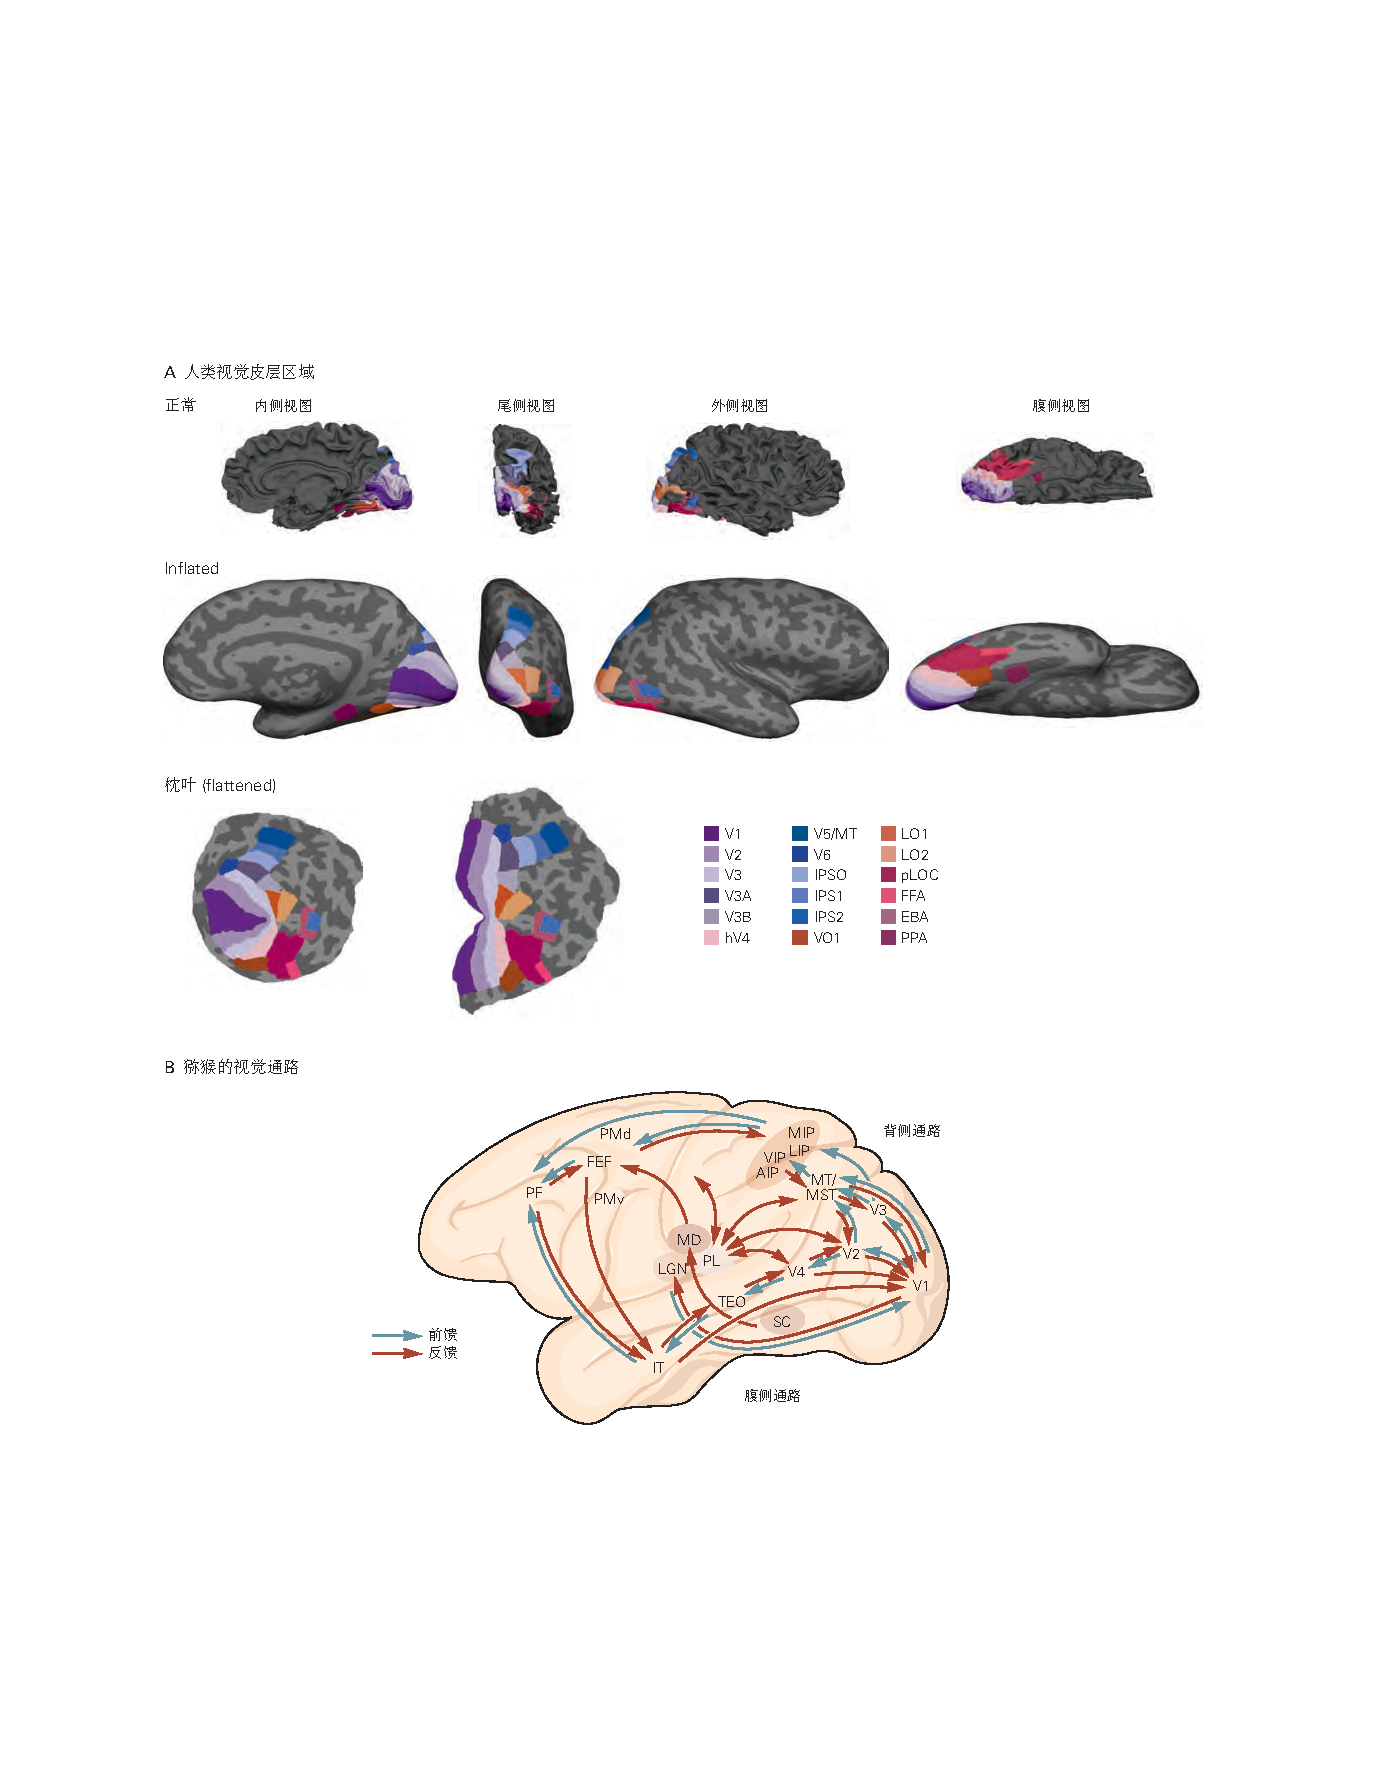
\includegraphics[width=0.95\linewidth]{chap21/fig_21_7}
	\caption{大脑皮层中的视觉通路。
		\textbf{A.} 功能磁共振成像显示了人类大脑皮层参与视觉处理的区域。
		顶行显示大脑正常视图的脑回和脑沟区域;
		中间一行显示了大脑的“膨胀”视图,该计算过程模拟大脑像气球一样膨胀,以便将脑回和脑沟的“皱纹”拉伸成光滑的表面,同时最大限度地减少局部变形。
		浅灰色和深灰色区域分别代表脑回和脑沟; 底行显示了枕叶的二维表示(左)和通过沿距状裂进行切割而失真较小的表示。
		划分不同的功能区域需要不同的方法。
		根据定义,视网膜区域包含视觉空间的连续图,并使用诸如旋转螺旋或扫过视觉空间的扩大圆圈等刺激来识别。
		相邻皮层区域的地图在皮层表面以相反的方向运行,并沿着局部镜像反转的边界相遇。
		这些镜像反转可用于识别区域边界,从而划分每个区域。
		这些视网膜专题区域,包括早期视觉区域 V1、V2 和 V3,以及区域 V3A、V3B、V6、hV4、VO1、LO1、LO2 和 V5/\textit{内侧颞叶},成对共享边界; 这些边界在枕骨极汇聚(在中央凹的代表处)。
		一种不同的方法,识别注意位点,用于映射区域 IPS1 和 IPS2。
		然而,对特定属性或目标类别(例如面部)的进一步方法或响应性用于不太严格的视网膜区域。
		许多视觉区域的功能特异性已得到证实:VO1 与颜色处理有关,外侧枕骨复合体(LO2,pLOC)编码物体形状,\textit{梭状回面孔区}编码面部,\textit{海马旁回}响应更多 对地方的反应比对物体的反应强烈,\textit{纹外体区域}对身体部位的反应比对物体的反应更强烈,并且 V5/\textit{内侧颞叶}参与运动处理。
		顶内沟(IPS1 和 IPS2)中的区域参与空间注意力和扫视眼球运动的控制。
		\textbf{B.} 在猕猴中,初级视觉皮层位于枕叶表面,并通过两条通路发送轴突。
		背侧通路穿过顶叶的多个区域并进入额叶,并调节注意力控制和视觉引导运动。
		腹侧通路通过 V4 投射到下颞皮层区域并介导物体识别。
		除了从初级视觉皮层延伸到颞叶、顶叶和额叶(蓝色箭头)的前馈通路外,相互或反馈通路在相反方向运行(红色箭头)。
		前馈和反馈可以在皮层区域之间直接运行,或通过丘脑间接运行,特别是丘脑,它充当皮层区域之间的中继。 
		涉及的皮层下通路包括丘脑核(\textit{外侧膝状体核}、\textit{枕核}和\textit{背内侧核})以及\textit{上丘}。}
	\label{fig:21_7}
\end{figure}


皮层的视觉区域可以通过其神经元的功能特性来区分。
对此类功能特性的研究表明,视觉区域分为两个等级通路,一个涉及物体识别的腹侧通路和一个专门用于使用视觉信息指导运动的背侧通路。
腹侧或物体识别通路从初级视觉皮层延伸到颞叶;
它在第~\ref{chap:chap24}~章中有详细描述。
背侧或运动引导通路将初级视觉皮层与顶叶连接,然后与额叶连接。


这些路径是相互连接的,因此可以共享信息。
例如,背侧通路中的运动信息可以通过运动学线索促进物体识别。
因此,来自背侧通路区域的空间运动信息对于物体形状的感知很重要,并被馈送到腹侧通路。


皮层区域之间的所有连接都是相互的,即每个区域都会将信息发送回它接收输入的区域。
这些反馈连接向早期视觉处理水平提供有关认知功能的信息,包括空间注意力、刺激预期和情感内容。
丘脑中的枕作为皮层区域之间的中继(见图~\ref{fig:21_7}B)。


背侧通路穿过顶叶皮层,该区域使用视觉信息来指导眼睛和四肢的运动,即视觉运动整合。
侧顶内区域因其位于顶内沟中而得名,参与表示空间中的点,这些点是眼球运动或到达的目标。
顶叶区域受损的患者无法注意身体一侧的物体,这种综合症称为单侧忽视(参见第~\ref{chap:chap59}~章图~\ref{fig:59_1})。


腹侧通路延伸到颞叶。
下颞皮层存储有关物体形状和身份的信息;
一部分代表面孔,因为该区域受损会导致无法识别面孔(面容失认症)。


背侧和腹侧通路各自包含一系列可以通过几个标准来描述的区域。
首先,在许多中继站,输入阵列形成了视觉半场的地图。 
这些地图的边界可以用来标定可视区域的边界。
这在通路的早期水平特别有用,在这些通路中,神经元的感受野很小,视觉主题图被精确组织(感受野的定义见下一节)。
然而,在更高的层次上,接受域变得更大,地图更不精确,因此视觉主题组织成为描绘区域边界的可靠基础。


另一种将一个区域与另一个区域区分开来的方法,如猴子实验所示,取决于每个区域的神经元所表现出的独特功能特性。
最明显的例子是背侧通路中的一个区域,即\textit{内侧颞叶},其中包含的神经元对穿过其感受野的运动方向具有很强的选择性。
与中间颞区参与运动分析的观点一致,该区域的病变会导致跟踪移动物体的能力下降。


视觉皮层区域组织的经典观点是层次结构,其中层次结构底部的区域,如初级视觉皮层和次级视觉皮层,代表方向、运动方向、深度和颜色的视觉原语。
在这个观点中,腹侧通路层次结构的顶部代表整个物体,中间区域代表中层视觉。
这种沿着层次结构“复杂化”的想法表明了视觉感知水平与皮层区域序列阶段之间的映射。
但最近的研究结果表明了一个更复杂的故事,即使是初级视觉皮层也在中层视觉中发挥作用,而较高区域的神经元可能会处理有关物体成分的信息。
此外,如图~\ref{fig:21_7}~所示,还必须考虑到这样一个事实,即从“较高”皮层区域到“较低”皮层区域存在强大的信息反向流动或反馈。
正如将在第~\ref{chap:chap23}~章中描述的那样,这种反向信息包含更高阶的“自上而下”认知影响,包括注意力、目标期望、知觉任务、知觉学习和效应复制。
自上而下的影响可能在场景分割、目标关系和目标细节感知以及目标识别本身中发挥作用。



\section{视觉通路中连续中继的神经元的感受野为大脑如何分析视觉形式提供了线索}

1906 年,\textit{查尔斯$\cdot$谢林顿}在他对刮擦退缩反射的分析中创造了感受野一词:“可以引发刮擦反射的皮肤表面点的整个集合称为该反射的感受野。” 
当可以从眼睛中的单个神经元进行记录时,\textit{霍尔登$\cdot$凯弗$\cdot$哈特兰}在他对鲎视网膜的研究中应用了感受野的概念:“必须照亮的视网膜区域才能在任何给定的纤维中获得响应。
被称为该纤维的感受野。” 
在视觉系统中,神经元的感受野代表视野中的一个小窗口(图~\ref{fig:21_8})。


\begin{figure}[htbp]
	\centering
	\includegraphics[width=1.0\linewidth]{chap21/fig_21_8}
	\caption{与光感受器相关的视网膜神经节细胞的感受野。
		\textbf{A.} 对视网膜神经节细胞感受野有贡献的光感受器的数量因感受野在视网膜上的位置而异。
		中央凹附近的细胞接收来自覆盖较小区域的较少受体的输入,而远离中央凹的细胞接收来自覆盖较大区域的更多受体的输入(见图~\ref{fig:21_10})。
		\textbf{B.} 光线穿过神经细胞层到达视网膜后部的光感受器。
		来自光感受器的信号随后由外核层和内核层中的神经元传输到视网膜神经节细胞。}
	\label{fig:21_8}
\end{figure}


但是,仅对一个光点的反应导致对细胞感受野的了解有限。
\textit{哈特兰}和研究哺乳动物视网膜的\textit{斯蒂芬$\cdot$库夫勒}使用两个小光点,在感受野中发现了抑制性环绕或\textit{侧抑制}区域。
1953 年,\textit{库夫勒}观察到“不仅可以通过视网膜照明实际建立反应的区域可以包含在感受野的定义中,而且还可以包括所有显示功能连接的区域,通过对视网膜的抑制或兴奋作用。” 
因此,\textit{库夫勒}证明了视网膜神经节细胞的感受野具有功能不同的分区。
这些感受野有一个中心环绕的组织,属于两类之一:在中心和偏离中心。
后来的工作表明,外侧膝状体中的神经元具有相似的感受野。


当圆形中心区域内的光点打开时,中心细胞就会发光。
当感受野中心的一个光点被关闭时,偏离中心的细胞就会放电。
周围的环形区域具有相反的符号。 
对于中心细胞,当光关闭时,中心周围环状空间中任何地方的光刺激都会产生响应,这种响应称为中心、非环绕。 
中心和周围区域相互抑制(图~\ref{fig:21_9})。
当中心和周围都被漫射光照射时,几乎没有或没有反应。 
相反,感受野的明暗边界会产生活跃的反应。
因为这些神经元对边界和轮廓最敏感(对照明差异而不是均匀表面),它们编码有关视野中对比度的信息。


\begin{figure}[htbp]
	\centering
	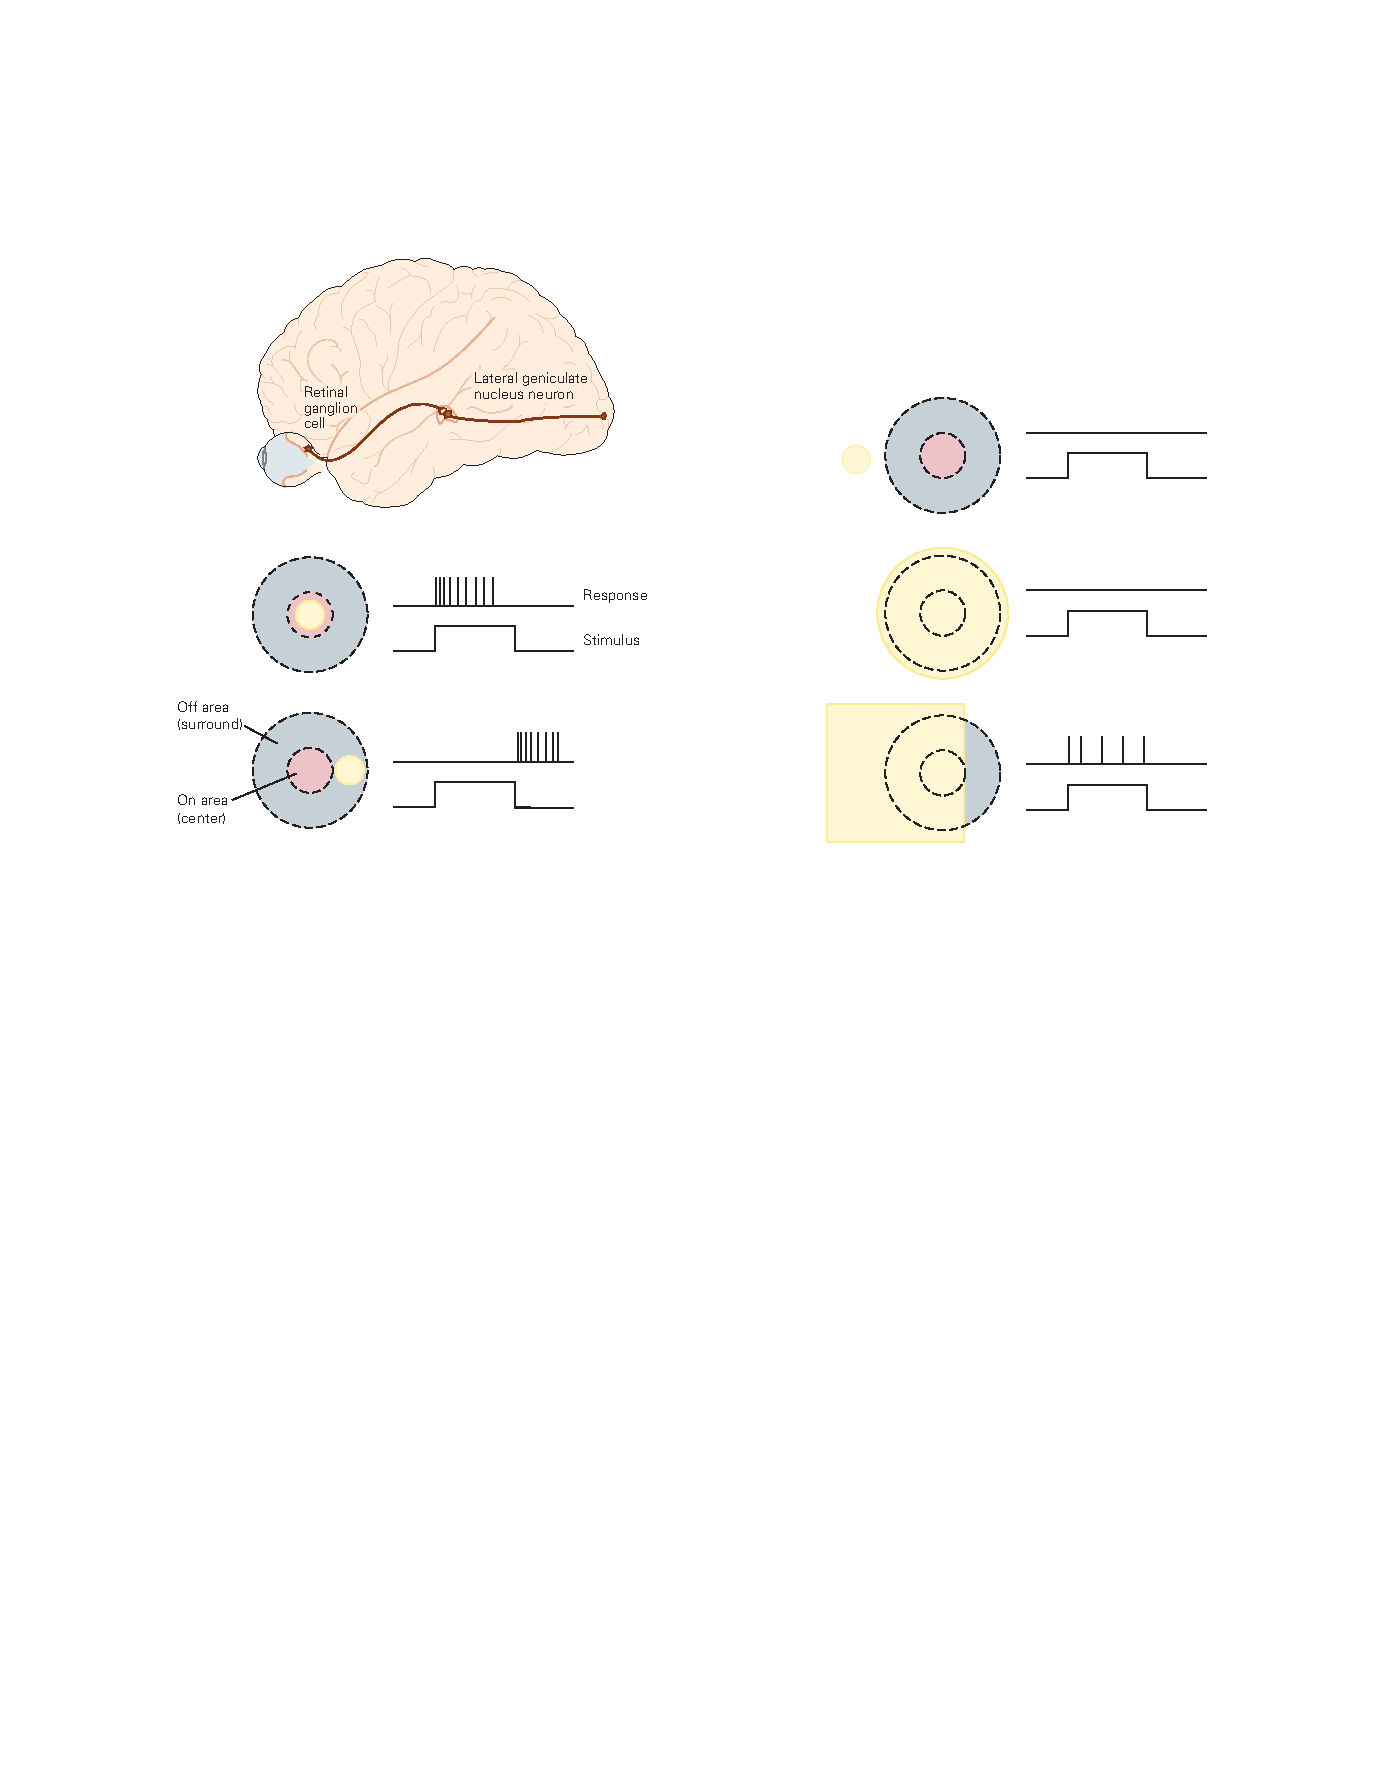
\includegraphics[width=1.0\linewidth]{chap21/fig_21_9}
	\caption{视觉通路早期中继神经元的感受野。
		具有相互对立的中心和周围的圆形对称感受野是丘脑外侧膝状体核中视网膜神经节细胞和神经元的特征。
		中心可以响应光点(黄色)的打开或关闭,具体取决于接收场分别属于“在中心”还是“偏离中心”类。
		环绕声有相反的反应。
		在环绕之外,对光没有反应,从而定义了感受野边界。
		当光线同时覆盖中心和周围时,反应较弱,因此这些神经元对视野中的对比度(明暗边界)做出最佳反应。}
	\label{fig:21_9}
\end{figure}


感受野在视网膜上的大小根据感受野的偏心率(它相对于中央凹的位置,视网膜中央部分视力最高的位置)和视觉通路上神经元的位置而变化。
具有相同偏心率的感受野在视觉处理的早期阶段相对较小,在后期阶段逐渐变大。
感受野的大小用视角的度数表示;
整个视野覆盖近 180°(图~\ref{fig:21_10}A)。
在视觉处理的早期中继中,中央凹附近的感受野是最小的。
监测中央凹部分的视网膜神经节细胞的感受野大约为 0.1°,而视觉周边的感受野可能大几个数量级。


\begin{figure}[htbp]
	\centering
	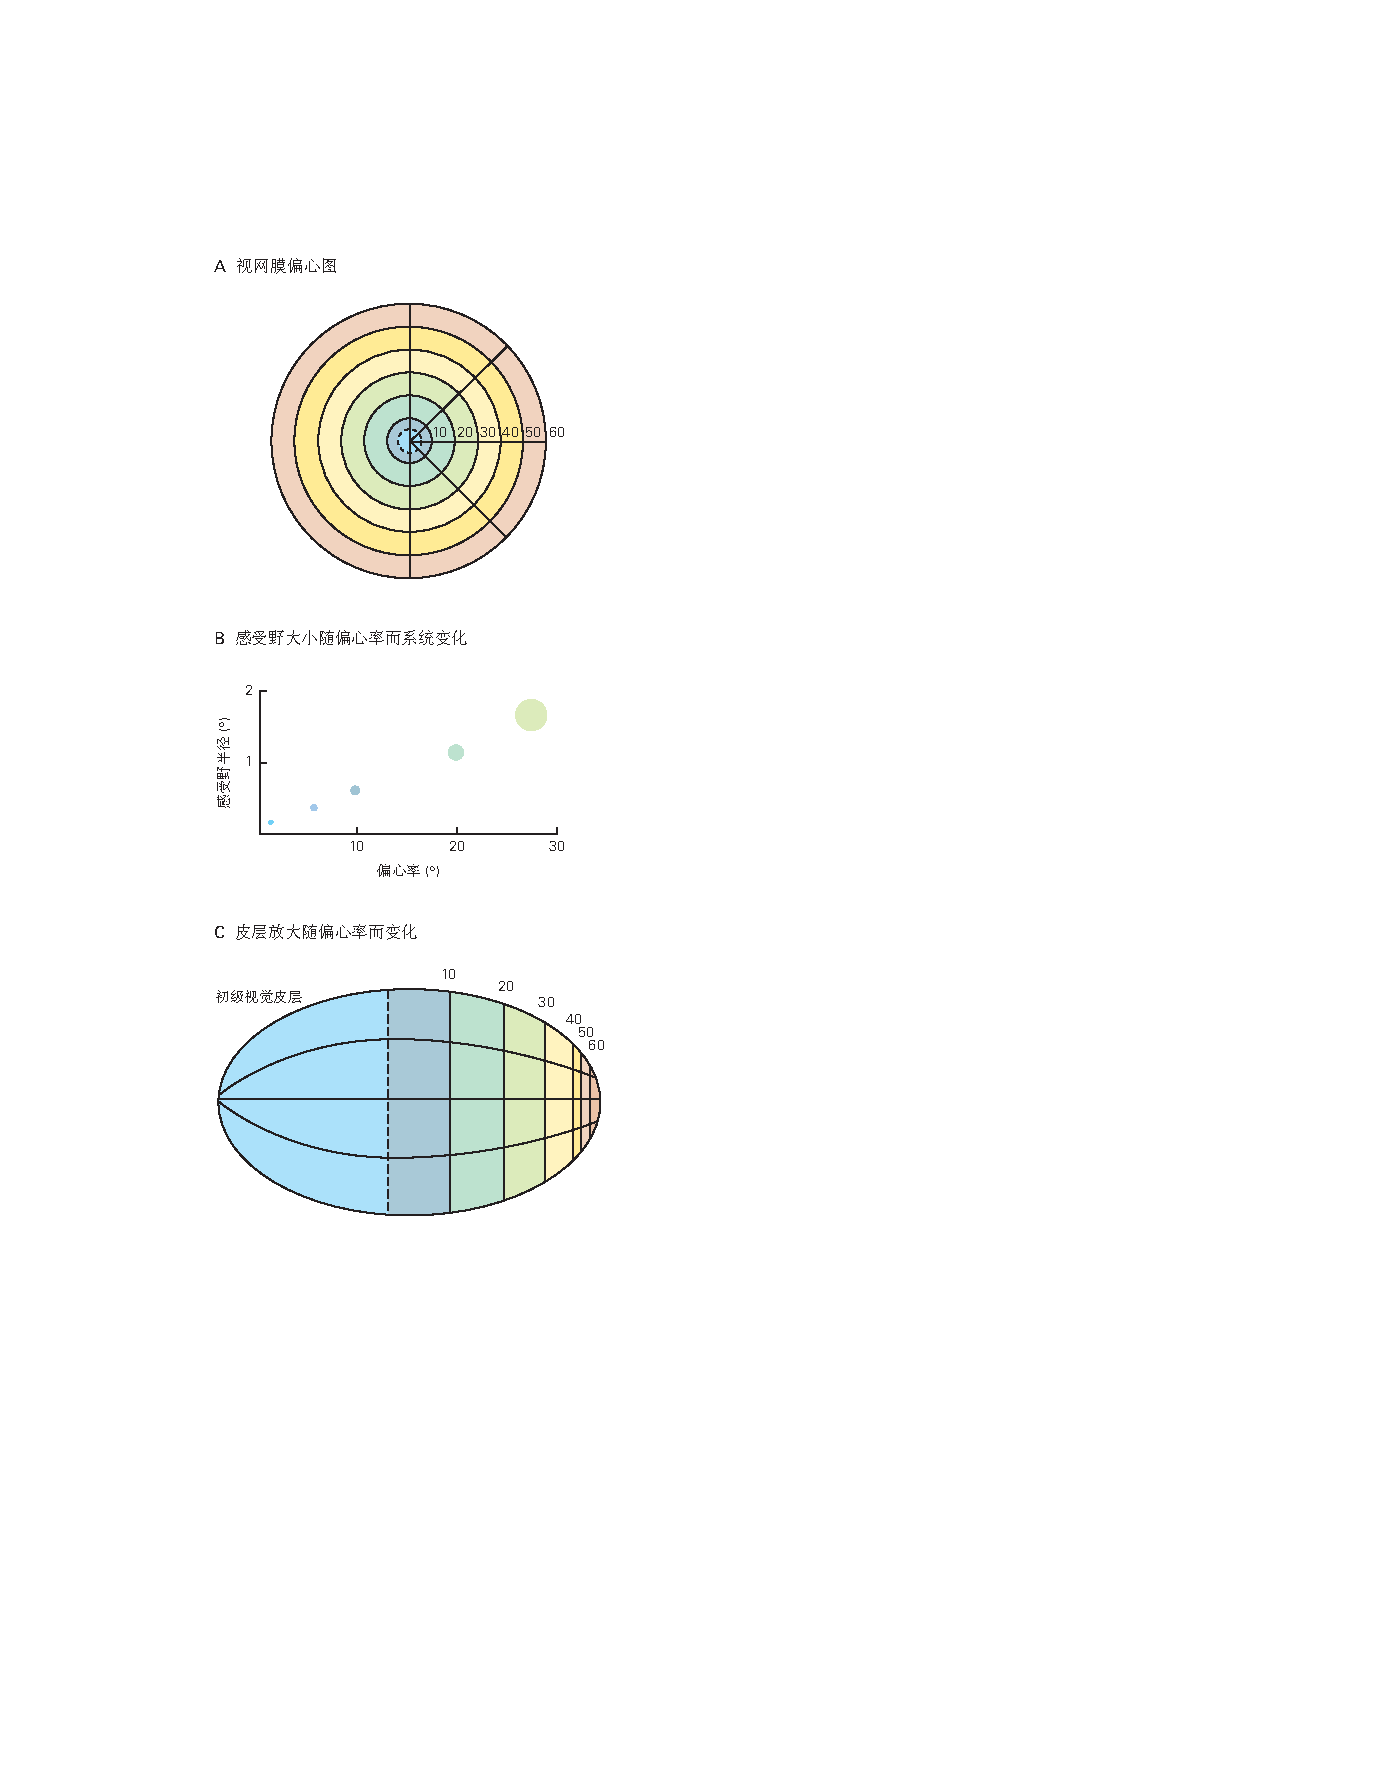
\includegraphics[width=0.55\linewidth]{chap21/fig_21_10}
	\caption{感受野大小、偏心率、视网膜组织和放大倍数。
		颜色编码指的是视觉空间或视网膜上的位置。
		\textbf{A.} 感受野与中央凹的距离称为感受野的偏心率。
		\textbf{B.} 感受野大小随与中央凹的距离而变化。
		最小的视场位于注视中心,即中央凹,视觉分辨率最高;
		视场随着距中央凹的距离逐渐变大。
		\textbf{C.} 专用于每个视觉空间度数内输入的皮层区域的数量,称为放大因子,也随偏心率而变化。
		视野的中央部分控制着最大的皮层区域。
		例如,在初级视觉皮层中,更多的区域专用于视觉空间的中心 10°,而不是其他所有区域。
		V1 的地图显示皮层片展开。}
	\label{fig:21_10}
\end{figure}


专用于一定程度视觉空间的皮层数量随偏心率而变化。
更多的皮层区域专用于视野的中央部分,那里的感受野最小,视觉系统具有最大的空间分辨率(图~\ref{fig:21_10}C)。


感受野属性会随着视觉通路的中继而变化。
通过确定这些特性,可以分析每个中继核的功能以及大脑如何逐步分析视觉信息。
例如,发生在外侧膝状体和大脑皮层之间的感受野结构的变化揭示了大脑分析视觉形式的重要机制。
形式路径的关键属性是对视野中轮廓方向的选择性。
这是初级视觉皮层信号处理的涌现特性;
它不是皮层输入的属性,而是在皮层本身内产生的。


外侧膝状体中的视网膜神经节细胞和神经元具有同心的中心环绕感受野,而皮层中的神经节细胞和神经元虽然对对比度同样敏感,但也会分析轮廓。
\textit{大卫$\cdot$休伯尔}和\textit{托斯坦$\cdot$威泽尔}于 1958 年在研究哪些视觉刺激会激发初级视觉皮层神经元的活动时发现了这一特征。
在展示包含各种图像的麻醉动物幻灯片时,他们从视觉皮层中的单个神经元进行细胞外记录。
当他们从一张幻灯片切换到另一张幻灯片时,他们发现了一个产生一系列快速动作电位的神经元。
细胞不是对载玻片上的图像有反应,而是对载玻片移动到位时的边缘有反应。



\section{视觉皮层被组织成专门的神经元柱}

初级视觉皮层功能组织的主要特征是其细胞的视位组织:
视野在整个皮层表面系统地呈现(图~\ref{fig:21_11}A)。


\begin{figure}[htbp]
	\centering
	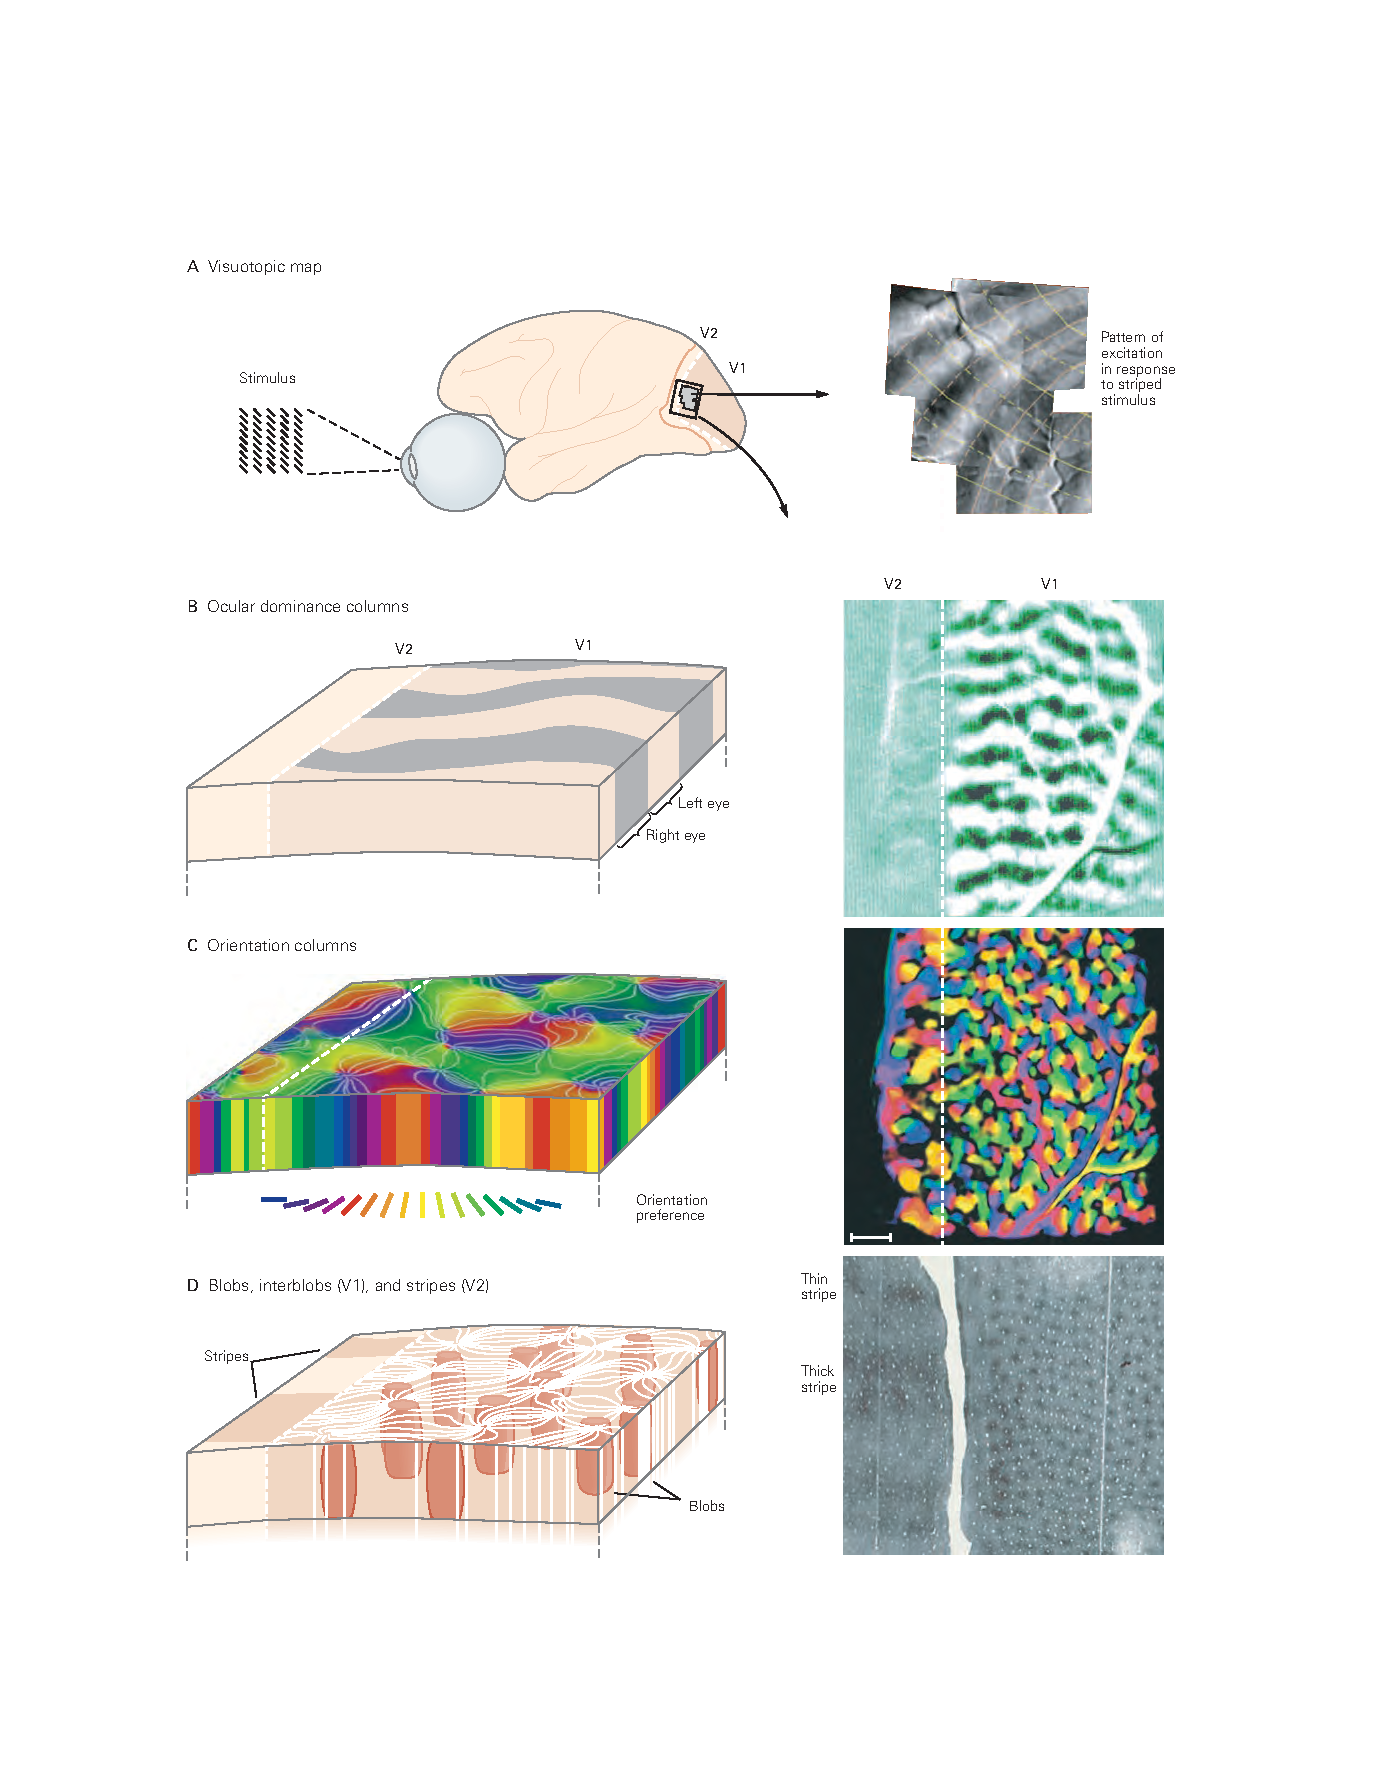
\includegraphics[width=0.95\linewidth]{chap21/fig_21_11}
	\caption{初级视觉皮层的功能结构。
		\textbf{A.} 初级视觉皮层的表面在功能上被组织为视野图。 
		视觉空间的仰角和方位角被组织在一个规则的网格中,由于放大系数的变化而扭曲(见图~\ref{fig:21_10})。
		此处的网格在深色条纹中可见(通过固有信号光学成像可视化),它反映了神经元对一系列垂直糖果条纹做出反应的模式。
		在此表面图中,人们发现了功能特定的细胞列的重复叠加循环,如 B、C 和 D. B 中所示。
		深色和浅色条纹代表左右眼优势列的表面视图。
		这些条纹以直角与区域初级视觉皮层和次级视觉皮层之间的边界相交,垂直子午线的表示。
		\textbf{C.} 一些列包含对刺激方向具有相似选择性的细胞。 
		不同的颜色表示列的方向偏好。
		表面视图中的方向列最好描述为围绕方向突然变化的奇点(风车的中心)的风车。比例尺代表 1 毫米。
		\textbf{D.} V1 中的斑点图案和 V2 中的条纹代表功能组织的其他模块。
		这些模式用细胞色素氧化酶可视化。}
	\label{fig:21_11}
\end{figure}


此外,初级视觉皮层中具有相似功能特性的细胞在从皮层表面延伸到白质的列中靠得很近。
这些列与在任何给定皮层区域中分析的功能特性有关,因此反映了该区域在视觉中的功能作用。
在初级视觉皮层中开发的特性包括方向特异性和两只眼睛输入的整合,这是通过每只眼睛输入的相对强度或眼优势来衡量的。


眼优势列反映了来自外侧膝状体不同层的丘脑皮层输入的分离。
该核的交替层接收来自位于同侧或对侧视网膜的视网膜神经节细胞的输入(图~\ref{fig:21_12})。
这种隔离在从外侧膝状体到初级视觉皮层的输入中得以维持,从而产生交替的左眼和右眼眼优势带(图~\ref{fig:21_11}B)。


具有相似方向偏好的细胞也被分组到柱中。
在整个皮层表面,方向偏好有规律的顺时针和逆时针循环,整个 180° 循环每 750 微米重复一次(图~\ref{fig:21_11}C)。
同样,左眼和右眼优势列以 750 到 1 千微米的周期交替。
一个完整的方向列循环,或一对完整的左眼和右眼优势列,称为超列。
皮层表面上每个点的方向和眼优势列在局部大致相互正交。
因此,一个皮层块一个超列的范围包含方向偏好和左眼和右眼优势的所有可能组合。


两种类型的列首先通过记录神经元在皮层中紧密间隔的电极穿透处的反应来绘制。
还通过在外侧膝状体的各个层中进行损伤或示踪剂注射来识别眼优势列。
最近,一种称为光学成像的技术使研究人员能够可视化活体动物的方向和眼优势柱的表面表示。 
该技术由\textit{阿米拉姆$\cdot$格林弗德}为研究皮层组织而开发,可视化与活跃的神经元群的代谢需求相关的表面反射率的变化,称为固有信号光学成像,或电压敏感染料的荧光变化。 
内在信号成像取决于局部血流中与活动相关的变化以及血红蛋白和其他内在发色团氧化状态的改变。 
这些技术现在还与使用基因编码的神经活动标记的细胞分辨率成像相辅相成。


实验者可以可视化具有左眼或右眼优势的细胞分布,例如,通过从刺激另一只眼睛时获得的图像中减去刺激一只眼睛时获得的图像。 
当在与皮层表面相切的平面上观察时,眼优势柱显示为交替的左眼和右眼条纹,每条条纹的宽度约为 750 微米(图~\ref{fig:21_11} B)。


定向柱的循环形成各种结构,从平行条纹到风车。 
定向偏好的急剧跳跃发生在定向图中的风车中心和“裂缝”处(图~\ref{fig:21_11}C)。


嵌入在方向和眼优势列中的是神经元簇,它们的方向选择性差但颜色偏好强烈。
这些位于表层内的专业化单位由细胞色素氧化酶的组织化学标记揭示,细胞色素氧化酶以斑点和间斑的规则斑块模式分布。
在初级视觉皮层中,这些斑点的直径为几百微米,相距 750 微米(图~\ref{fig:21_11}D)。
斑点对应于颜色选择性神经元簇。
因为它们富含具有颜色选择性的细胞而缺乏具有方向选择性的细胞,所以这些斑点专门提供有关表面而不是边缘的信息。


在 V2 区,用细胞色素氧化酶标记可明显看出由浅色条纹分隔的粗细深色条纹(图~\ref{fig:21_11}D)。
粗条纹包含对运动方向和双眼视差有选择性的神经元,以及对虚幻轮廓和全局视差线索有反应的细胞。
细条纹容纳专门用于颜色的细胞。
浅色条纹包含定向选择性神经元。


对于要在视野中每个位置分析的每个视觉属性,必须有足够的平铺或覆盖具有不同功能特性的神经元。
当一个人在皮层表面的任何方向上移动时,感受野的视位位置的进展是渐进的,而列的循环发生得更快。
因此,可以通过单个计算模块根据轮廓的方向、物体的颜色和运动方向以及立体深度来充分分析视野中的任何给定位置。
包含此类模块的一小部分视觉皮层代表所有柱状系统的所有可能值(图~\ref{fig:21_13})。


\begin{figure}[htbp]
	\centering
	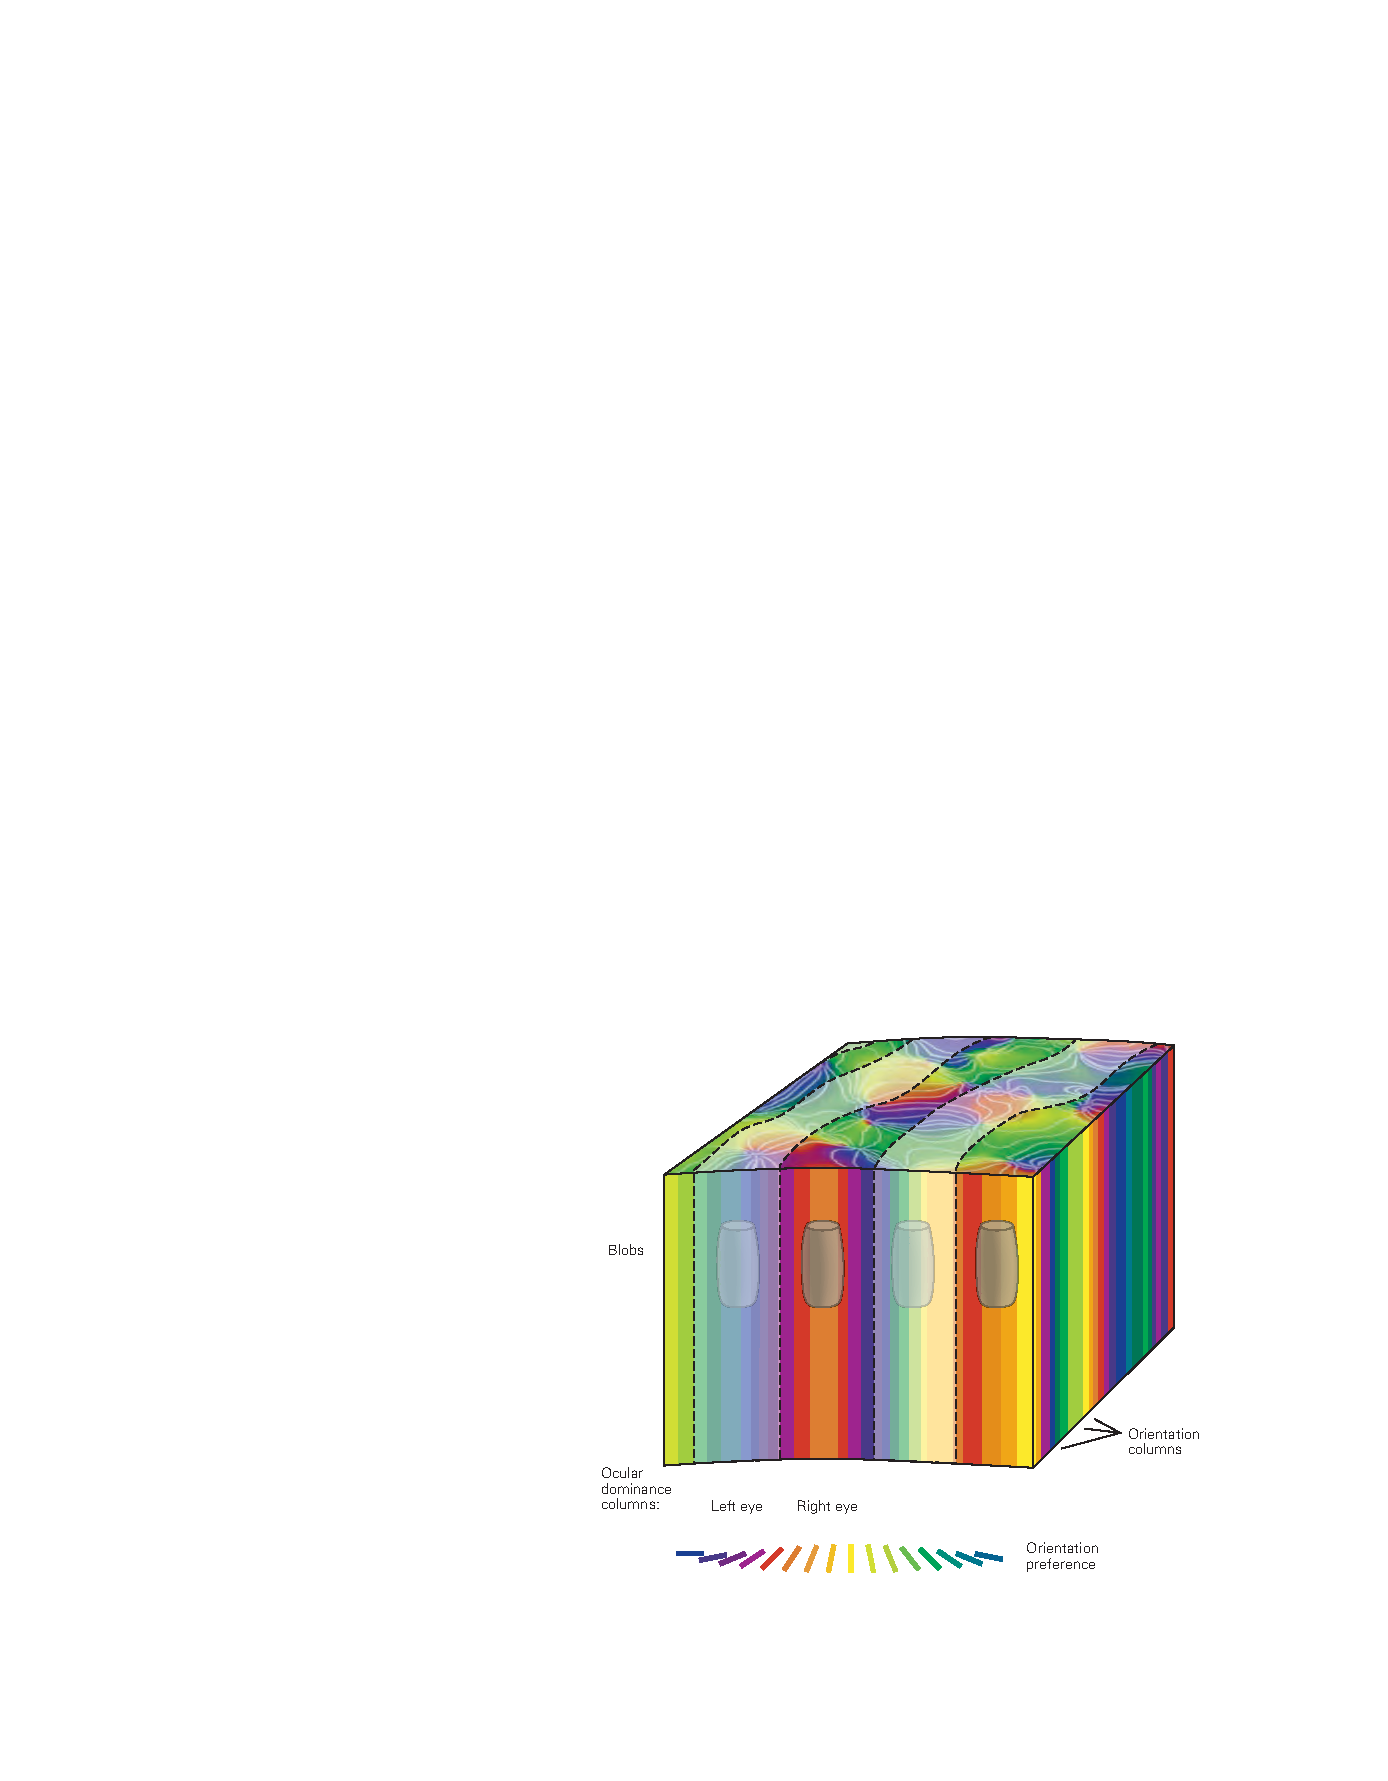
\includegraphics[width=0.75\linewidth]{chap21/fig_21_13}
	\caption{皮层计算模块。 
		一块大约 1 平方毫米的皮层组织包含一个定向超柱(一个完整的定向柱循环)、一个左眼和右眼优势柱循环,以及斑点和间斑。
		该模块可能包含初级视觉皮层的所有功能和解剖细胞类型,这些细胞将重复数百次以覆盖视野\cite{hubel1995eye}。}
	\label{fig:21_13}
\end{figure}


柱状系统充当沿着视觉通路的两种基本连接类型的基底。
串行处理发生在皮层区域之间的连续连接中,这些连接从大脑后部向前延伸。
同时,并行处理同时发生在处理不同子模态(如形状、颜色和运动)的纤维子集中,继续从视网膜开始的神经处理策略。


视觉皮层的许多区域都反映了这种排列;
例如,初级视觉皮层中功能特定的细胞与次级视觉皮层中具有相同特异性的细胞进行通信。
然而,这些路径并不是绝对隔离的,因为不同视觉属性之间存在一些信息混合(图~\ref{fig:21_14})。


\begin{figure}[htbp]
	\centering
	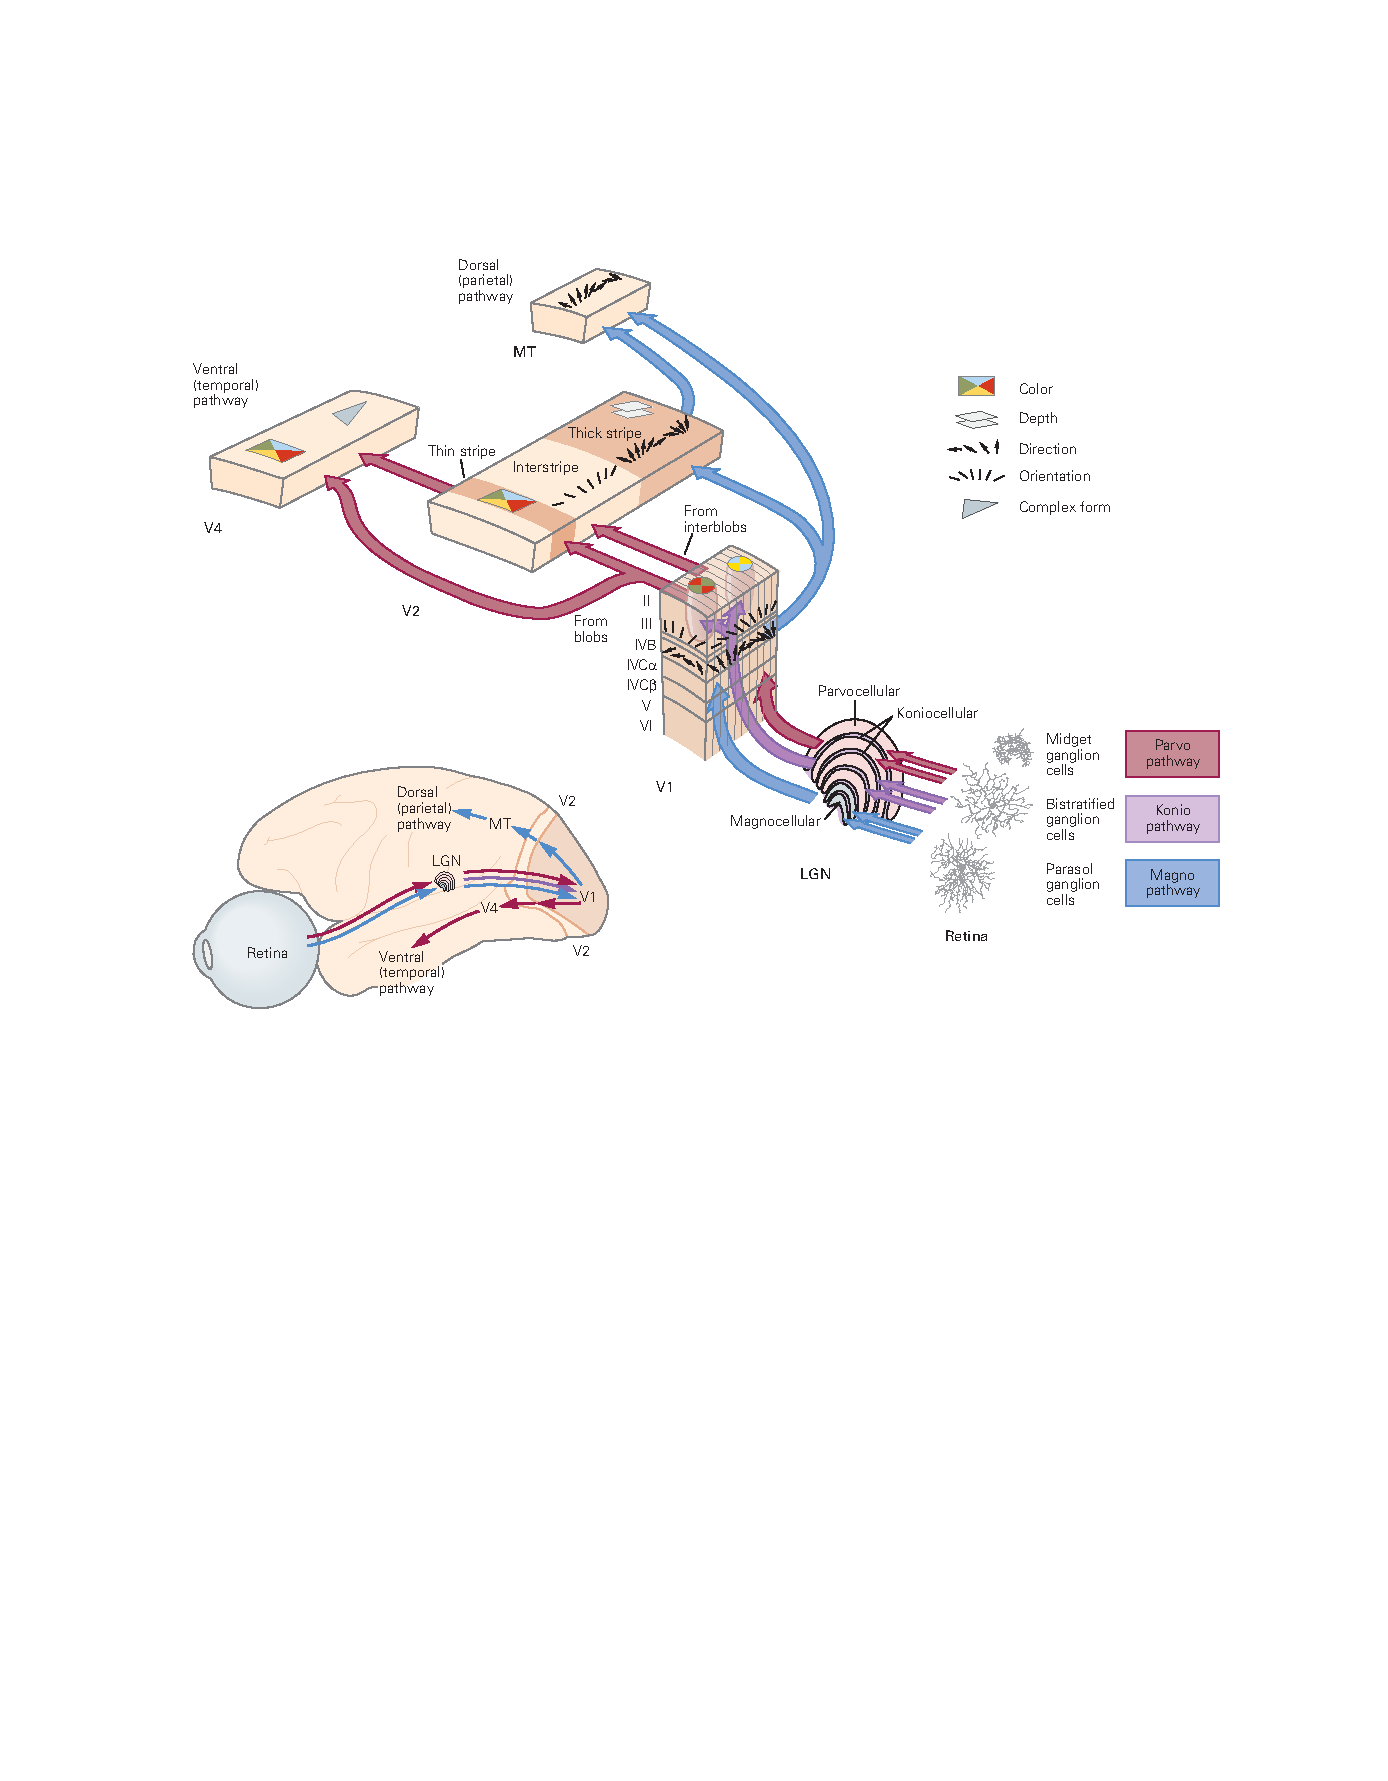
\includegraphics[width=1.0\linewidth]{chap21/fig_21_14}
	\caption{视觉通路中的并行处理。
		腹侧流主要与物体识别有关,携带有关形状和颜色的信息。
		背侧通路专用于视觉引导运动,细胞可选择运动方向。
		然而,这些通路并没有严格分开,即使在初级视觉皮层中,它们之间也存在实质性的相互联系。}
	\label{fig:21_14}
\end{figure}


柱状组织具有几个优点。
它最大限度地减少了具有相似功能特性的神经元相互通信所需的距离,并允许它们共享来自离散通路的输入,这些通路传递有关特定感觉属性的信息。
这种高效的连接节省了脑容量的使用,并最大限度地提高了处理速度。
将神经元聚集成功能组,就像在皮层的列中一样,可以使大脑最大限度地减少分析不同属性所需的神经元数量。
如果所有神经元都针对每个属性进行调整,那么由此产生的组合爆炸将需要数量惊人的神经元。



\section{内在皮层回路转换神经信息}

视觉皮层的每个区域都将眼睛收集并在较早的突触中继中处理的信息转换为代表视觉场景的信号。
这种转变是由包含兴奋性和抑制性神经元的局部回路完成的。


初级视觉皮层的主要输入来自三个平行通路,它们起源于\textit{外侧膝状体}的\textit{粒状}层的小细胞、大细胞和蓝色/黄色通道(见图~\ref{fig:21_12})。
小细胞层中的神经元投射到皮层 IVC$\beta$ 和 6 层,大细胞层中的神经元投射到 IVC$\alpha$ 层和第 6 层,而\textit{粒状}神经元投射到第 1 层和第 2 层和第 3 层中的细胞色素氧化酶斑点。
从那里开始,一个序列 由兴奋性多刺星状神经元介导的层间连接,通过一组刻板的连接处理视觉信息(图~\ref{fig:21_15})。


\begin{figure}[htbp]
	\centering
	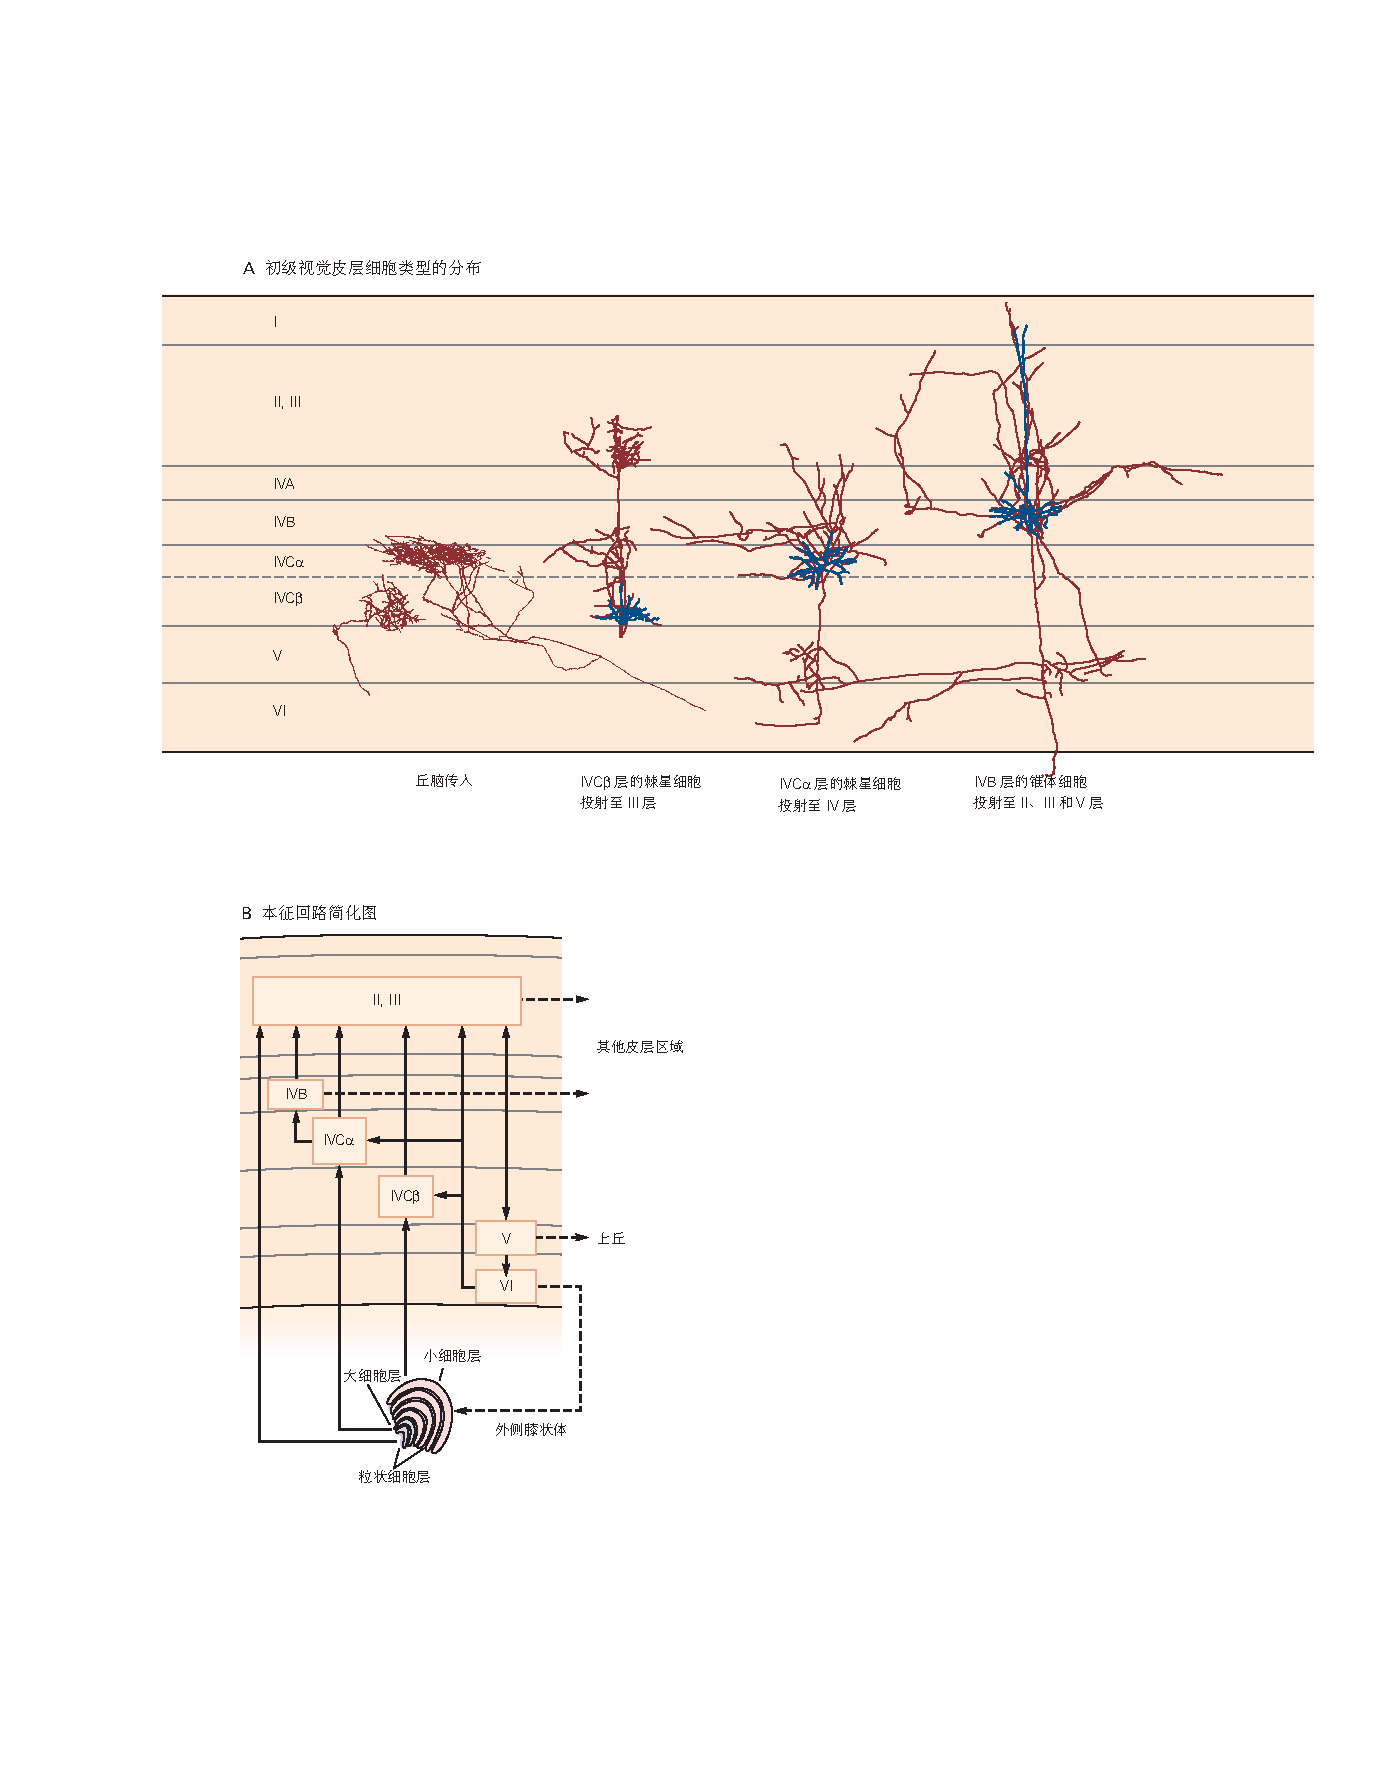
\includegraphics[width=1.0\linewidth]{chap21/fig_21_15}
	\caption{初级视觉皮层的内在回路。
		\textbf{A.} 不同皮层中负责皮层回路兴奋性连接的神经元示例。 
		第四层是来自丘脑外侧膝状体核的主要输入层。 
		来自细小细胞层的纤维终止于 IVC$\beta$ 层,而大细胞纤维终止于 IVC$\alpha$ 层。 
		内在皮层兴奋性连接由多刺星状细胞和锥体细胞介导。 
		多种 \textit{$\gamma$-氨基丁酸}能平滑星状细胞(未显示)负责抑制连接。 
		树突乔木是蓝色的,轴突乔木是棕色的\cite{blasdel1983termination}。
		\textbf{B.} 初级视觉皮层内的兴奋性连接图。
		从视觉皮层的每一层发送到皮层其他区域的输出。}
	\label{fig:21_15}
\end{figure}


并行通路的这种表征只是一种近似,因为通路之间存在相当大的相互作用。
这种交互是将各种视觉特征(颜色、形式、深度和运动)联系起来的方式,从而形成统一的视觉感知。
可以实现这种联系或绑定的一种方式是通过调整到多个属性的细胞。


在皮层处理的每个阶段,锥体神经元将输出扩展到其他大脑区域。
表层细胞负责连接到皮层的高阶区域。
第五层锥体神经元投射到脑干中的上丘和脑桥。
第六层细胞负责向丘脑和低阶皮层区域的反馈投射。


不同层的神经元具有不同的感受野特性。
初级视觉皮层表层神经元的感受野较小,而深层神经元的感受野较大。
表层神经元专门用于高分辨率模式识别。 
更深层的神经元,例如对运动方向具有选择性的第五层神经元,专门用于跟踪空间中的物体。


反馈投射被认为提供了一种途径,使路径中的较高中心可以影响较低中心。
从皮层投射到外侧膝状体的神经元数量是从外侧膝状体投射到皮层的神经元数量的 10 倍。
尽管这种反馈投射显然很重要,但其功能在很大程度上是未知的。


介导信息流入或流出皮层区域的兴奋性锥体和多棘星状神经元的活动也受到抑制性中间神经元局部网络的严格控制。
兴奋性神经元的尖峰率通过匹配抑制不断非线性平衡,从而保持神经对输入反应的稳定性。
抑制性中间神经元分为多个类别,其形态和不同肽(如小清蛋白、生长抑素或\textit{血管活性肠肽})的共表达不同。
其中一些中间神经元形成级联回路,其中一类中间神经元以另一类中间神经元为目标,然后再以兴奋性神经元为目标。
这导致神经回路中的多步控制机制,从而增加第一类抑制性中间神经元的活动会减少第二类的活动,从而在级联末端的兴奋性目标中解除抑制并增加反应。
这种抑制控制的基序可能对多个皮层感觉区域很常见。


除了串行前馈、反馈和局部循环连接之外,在每一层内平行于皮层表面行进的纤维还提供远程水平连接(图~\ref{fig:21_16})。
\textit{查尔斯$\cdot$吉尔伯特}和\textit{托斯坦$\cdot$威泽尔}分析了这些联系及其在皮层功能结构中的作用,他们使用细胞内记录和染料注射将解剖学特征与皮层功能相关联。
由于视觉皮层是按视觉局部组织的,因此水平连接允许目标神经元在相对较大的视野区域整合信息,因此对于将视觉图像的组成部分组装成统一的感知非常重要。


\begin{figure}[htbp]
	\centering
	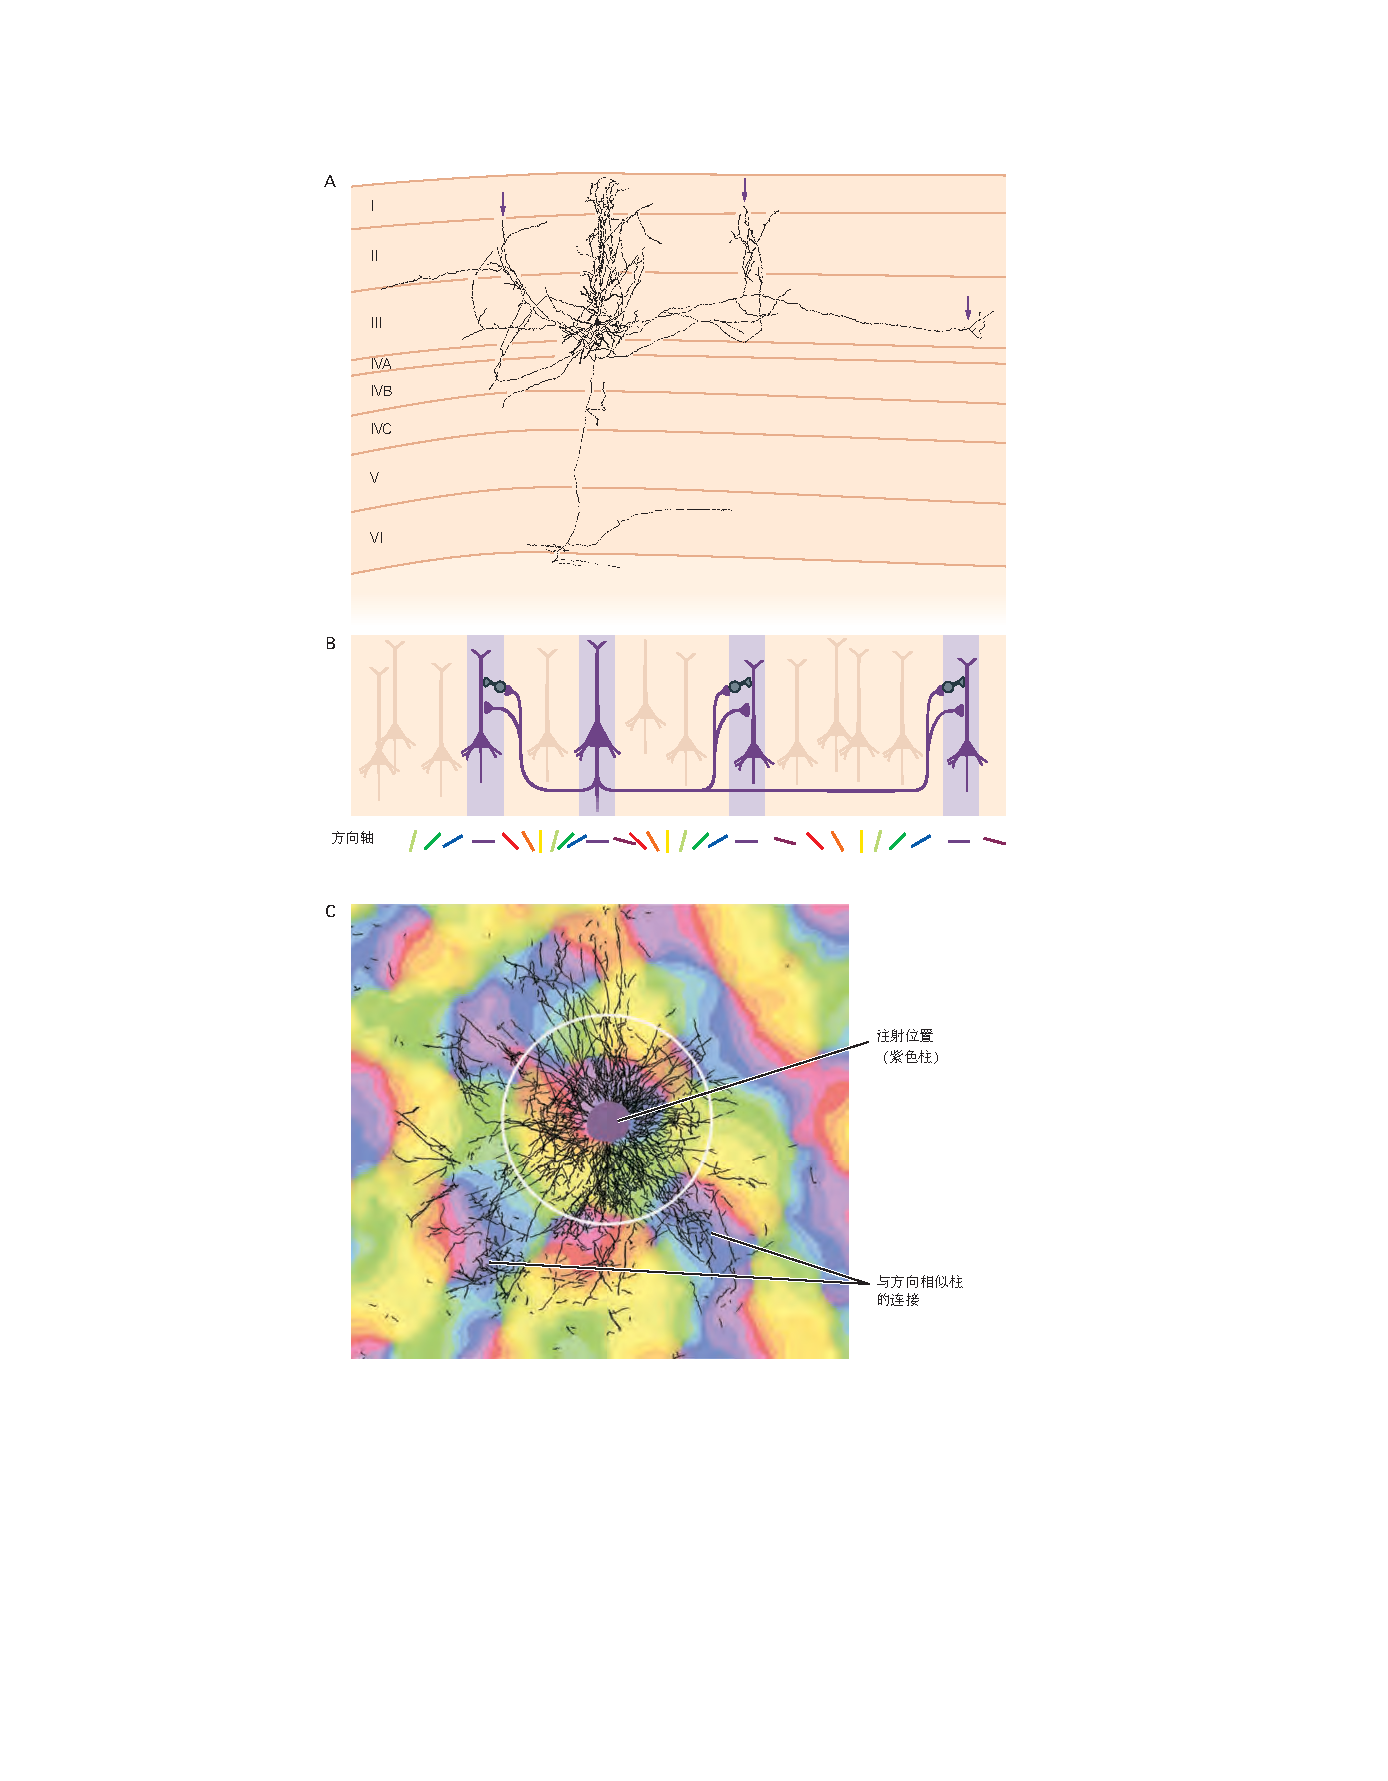
\includegraphics[width=0.75\linewidth]{chap21/fig_21_16}
	\caption{视觉皮层每一层的远程水平连接整合了来自视野不同部分的信息。
		\textbf{A.} 锥体细胞的轴突平行于皮层表面延伸数毫米。 
		轴突侧枝与其他锥体细胞以及抑制性中间神经元形成连接。
		这种安排使神经元能够整合大部分视野的信息。
		这些连接的一个重要特征是它们与功能列的关系。
		在距离细胞体大于 0.5 毫米的距离处,轴突侧支呈簇状(箭头)。
		\textbf{B.} 水平连接将具有相似方向特异性的细胞列连接起来。
		\textbf{C.} 通过将包含绿色荧光蛋白编码基因的腺病毒载体注入一个定向柱并将标记图像(黑色)叠加在注射附近定向柱的光学成像图上,可以看到水平连接的模式。(白色圆圈的直径为 1 毫米。)}
	\label{fig:21_16}
\end{figure}


集成也可以通过其他方式实现。
传入视觉通路的突触中继连接的相当大的收敛和发散意味着神经元的感受野在每个连续的中继上更大更复杂,因此具有整合功能。 
反馈连接也可能支持整合,这既是因为它们的分歧,也是因为它们起源于具有更大感受野的细胞。



\section{视觉信息由各种神经编码表示}

感觉通路中的单个神经元会对一系列刺激值做出反应。
例如,颜色检测通路中的神经元不限于响应一个波长,而是调谐到一系列波长。 
神经元的响应在特定值处达到峰值并在该值的两侧逐渐减弱,形成具有特定带宽的钟形调谐曲线。
因此,在 650 纳米处具有峰值响应且带宽为 100 纳米的神经元可能会在 600 纳米和 700 纳米处给出相同的响应。


为了能够确定神经元信号的波长,需要至少两个代表以不同波长为中心的滤波器的神经元。 
每个神经元都可以被认为是一条标记线,其中活动表示具有给定值的刺激。 
当不止一个这样的神经元发射时,突触后中继的会聚信号代表一种刺激,其波长是所有输入代表的值的加权平均值。


单个视觉感知是许多神经元活动的产物,这些神经元以特定的组合和交互方式运行,称为群体编码。 
群体编码已经以各种方式建模。 
最流行的模型称为向量平均。


我们可以用一群方向选择性细胞来说明群体编码,每个细胞都对具有特定方向的线作出最佳反应。 
每个神经元不仅对首选刺激作出反应,而且对落在具有特定带宽的高斯调谐曲线所描述的方向范围内的任何线作出反应。 
特定方向的刺激最强烈地激活调谐曲线以该方向为中心的细胞; 
调谐曲线远离该方向但与该方向重叠的细胞兴奋程度较低。


每个细胞的偏好方向,线标签,表示为指向该方向的向量。
每个细胞的放电都是对细胞线标签的“投票”,细胞的放电率代表投票的权重。
因此,细胞的信号可以用一个向量表示,该向量指向细胞的偏好方向,其长度与细胞响应的强度成正比。
对于所有激活的细胞,可以计算一个向量和,其方向代表刺激值(图~\ref{fig:21_17})。


\begin{figure}[htbp]
	\centering
	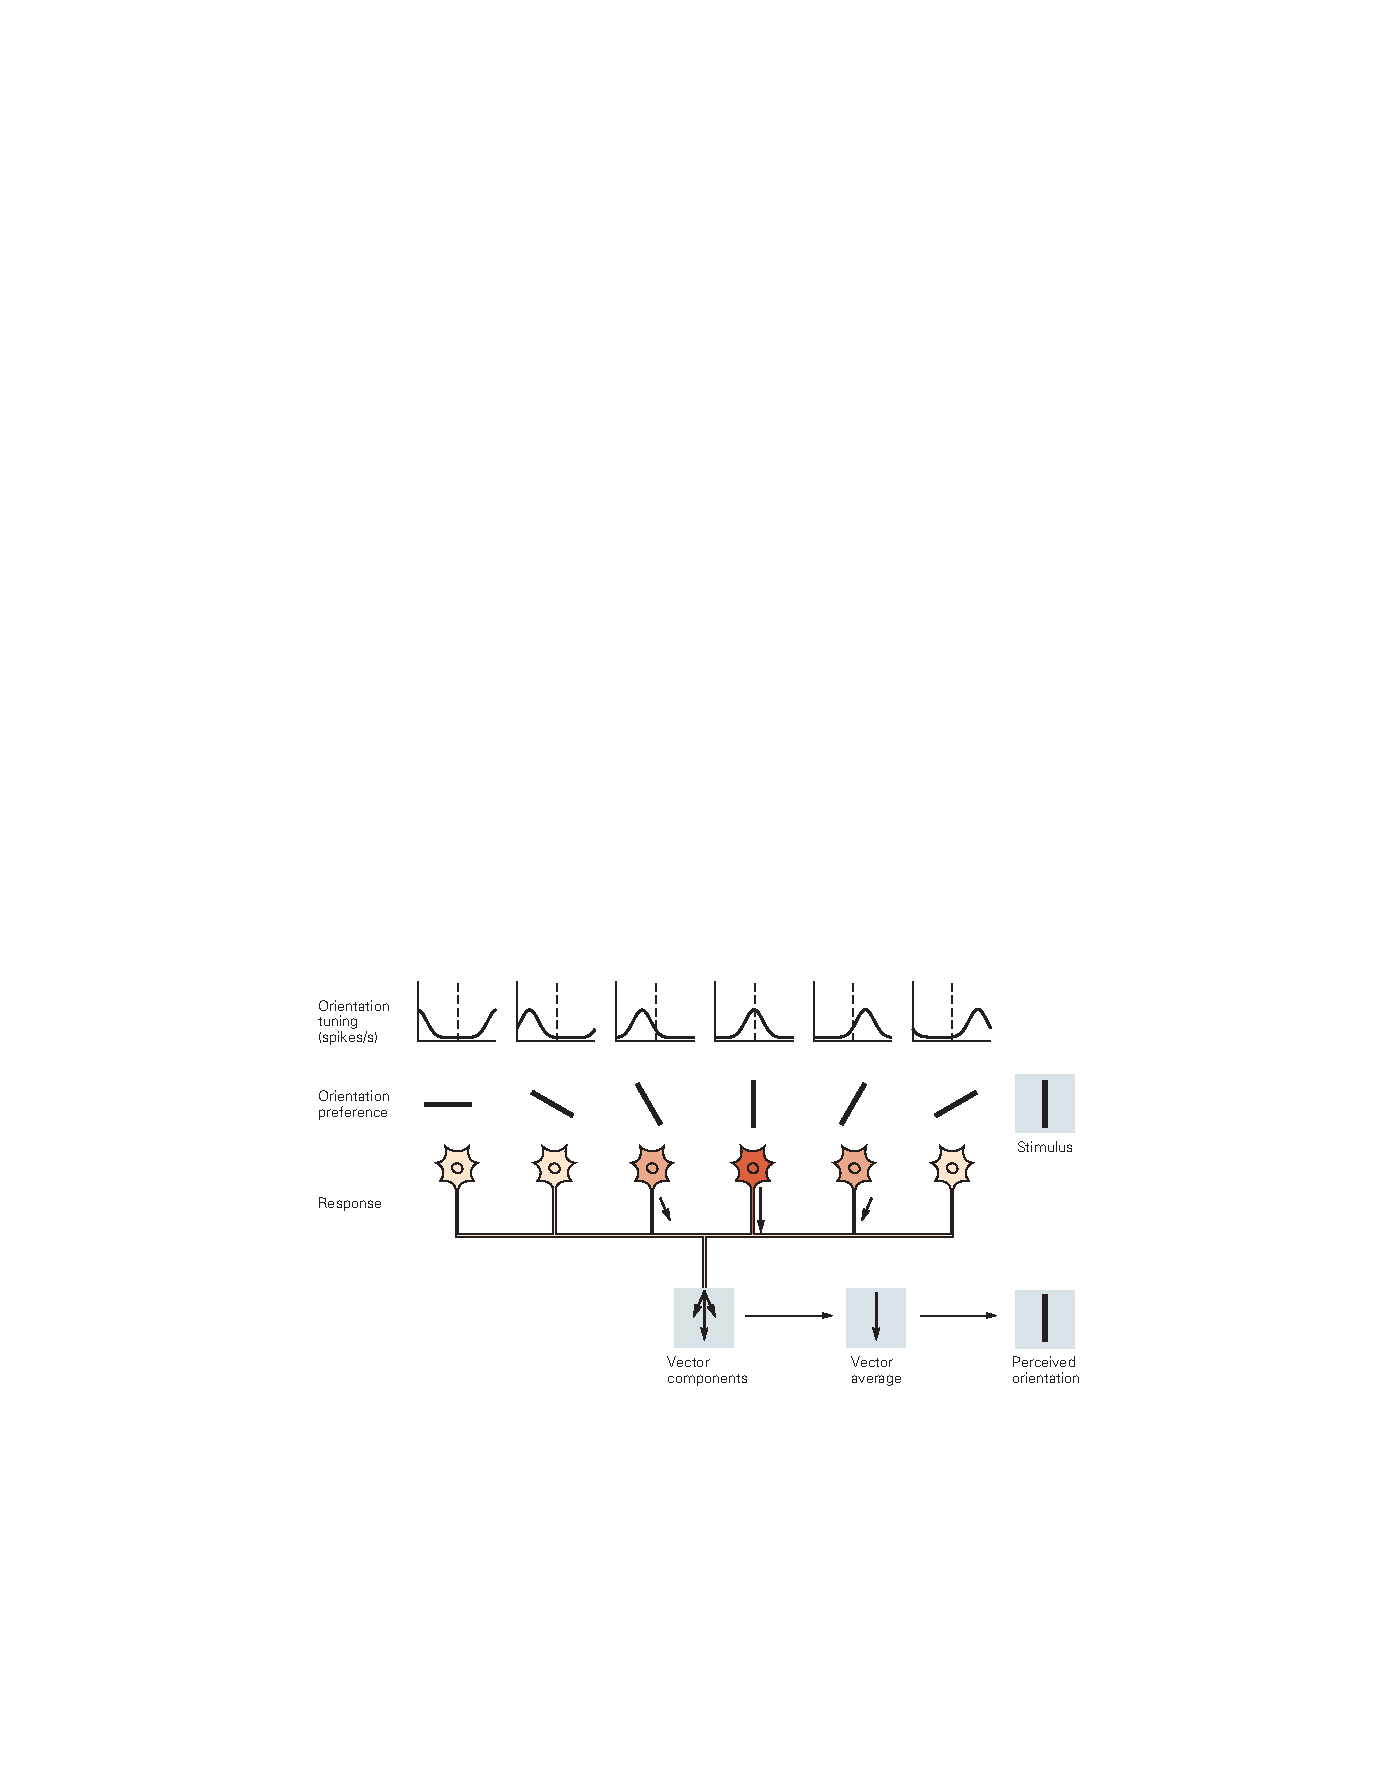
\includegraphics[width=1.0\linewidth]{chap21/fig_21_17}
	\caption{向量平均是神经回路中群体编码的一种模型。
		向量平均值描述了神经元集合中的响应、集合中单个神经元的调谐特性以及由此产生的感知之间的可能关系。
		单个神经元对视野中刺激的特定方向做出最佳反应,但也会以不同的速率对一系列方向做出反应。
		神经元最能激发的刺激方向可以被认为是一个线标签,当细胞快速激发时,它的活动表示存在具有该方向的刺激。
		许多具有不同方向偏好的神经元会对相同的刺激做出反应。
		每个神经元的响应都可以表示为一个向量,其长度表示其响应的强度,其方向表示其偏好方向或线标签\cite{kapadia2000spatial}。}
	\label{fig:21_17}
\end{figure}


群体密码的另一个方面是神经元对相同刺激的反应的可变性。
向对该刺激敏感的神经元重复呈现刺激将引发一系列响应。
神经元调谐曲线最敏感的部分不在峰值处,而是在调谐曲线最陡峭的两侧。
在这里,刺激值的微小变化会产生最强烈的反应变化。
然而,刺激值的变化必须足以引起明显超过神经元反应正常变异性的反应变化。
人们可以将该变化量与感知辨别阈值进行比较。
当许多神经元有助于辨别时,信噪比会增加,这一过程称为概率求和,并且神经元反应发生显著变化所需的刺激值的临界差异较小。


当大脑表示一条信息时,一个重要的考虑因素是参与该表示的神经元数量。
尽管有关视觉刺激的所有信息都存在于视网膜中,但视网膜表征不足以识别物体。
在视觉通路的另一端,颞叶中的一些神经元对复杂物体(例如面部)具有选择性。
一个单独的细胞能代表像一张特定面孔这样复杂的东西吗?
这样一个假设的神经元被称为“祖母细胞”,因为它完全代表一个人的祖母,或者被称为“教皇细胞”,因为它代表层次认知通路的顶点。


然而,神经系统并不能通过单个神经元的活动来代表整个目标。
相反,一些细胞代表物体的一部分,而一组神经元代表整个物体。
合奏中的每个成员都可以参与由不同目标激活的不同合奏。
这种安排被称为分布式编码。
分布式编码可能涉及几个或多个神经元。
在任何情况下,分布式编码都需要代表人脸的细胞与代表与该人相关的姓名和经历的细胞之间的复杂连接。


前面的讨论假设神经元通过它们的放电率和它们的线标签来传递信息。
另一种假设是动作电位的时间本身携带信息,类似于摩尔斯电码。
随着时间的推移,可以从不同神经元组的同步放电中读取编码。
在某一时刻,一组细胞可能会一起放电,然后另一组细胞同步放电。
通过一系列动作电位,单个细胞可以参与许多这样的集合。
感觉信息是否以这种方式表示,以及神经系统是否携带比仅由放电率表示的信息更多的信息,尚不清楚。



\section{亮点}

1. 视觉是一种建构过程,与照相机中单纯记录视觉输入有着根本的不同。
相反,大脑使用视觉输入来推断关于周围世界的信息,包括关于物体的信息,例如它们的大小、形状、距离和身份以及它们移动的速度。


2. 针对对比度、方向和运动等视觉特征的神经回路调整通常与自然环境中特征的分布相匹配。
这表明神经回路具有进化的、行为学驱动的起源。


3. 视觉回路和视觉是由个人视觉体验调节的。


4.视觉大量使用并行处理。
较高的视觉中心形成两条截然不同的通路。
位于顶叶皮层的背侧通路涉及运动知觉、注意力和视觉引导动作。
位于颞叶皮层的腹侧通路处理形状和物体。
腹侧通路的进一步细分是专门的,例如,用于识别面部。 
这些通路虽然截然不同,但却相互沟通;
这对于将物体视为连贯的整体可能很重要。
 

5. 并行处理始于视网膜。
不同的视网膜回路分析视觉输入每个点的不同局部特征,包括非彩色亮与暗、红色与绿色以及蓝色与黄色的局部对比。
信息通过不同类别的视网膜神经节细胞(针对上述三个特征,分别为大细胞、小细胞和\textit{粒状})发出,其轴突形成视神经。
 

6. 来自两只眼睛的视神经在视交叉处重新组合,使得来自左侧视觉半场的所有纤维都投射到大脑的右半球,反之亦然。
然而,平行的视网膜通道在解剖学上仍按眼睛和视觉特征隔离,经过丘脑中继站、外侧膝状体,直至初级视觉皮层。 


7. 不同的通道在不同的层进入初级视觉皮层,尽管它们主要在主要输入层 4 和 6 进入。
视觉输入被重新组合以提取新的特征集。
这些包括调整方向、运动和目标深度(通过组合左眼和右眼输入获得)。
 

8. 初级视觉皮层神经元共享空间位置或方向偏好等基本属性,形成从软脑膜垂直延伸到白质的柱。
 


9. 初级视觉皮层神经元还形成了它们在皮层上的反应特性的系统水平图。
对位置的调整形成了视觉空间的平滑“视觉拓扑”地图,它随着距离的增加而逐渐变化,并且在中央凹处得到最精细的分辨,向外围逐渐变得粗糙。
叠加在空间图上的是方向偏好和左眼与右眼偏好的局部平滑图,其中散布着优先处理颜色柱。
这些视觉反应特征在相对较短的皮层距离上循环,实际上在空间图的每个部分移动上完成一个完整的循环。
因此,初级视觉皮层回路有效地并行分析每个视觉位置,以获得全套初级视觉皮层视觉特征。 


10. 初级视觉皮层中的神经处理反映了它的架构,沿列的局部垂直处理和跨柱的横向处理。
此外,还有跨越多柱的远程处理。


11. 初级视觉皮层的输出逐渐进入更高的视觉区域,包括分布在背侧通路和腹侧通路的 30 多个中心。
连通性是相互的,较高的位点发送针对较低区域(包括外侧膝状体)的密集反馈。 


12. 视觉处理的一个有用衡量标准是视觉通路上神经元“感受野”的变化。
感受野是神经元接收输入的视觉空间区域;
它的进一步特征是神经元的最佳视觉刺激。
感受野在视觉通路的连续阶段变得更大、更复杂。
它们的最佳刺激也增加了复杂性,从用于光感受器的简单像素状点,到用于初级视觉皮层的定向线,再到位于腹侧通路更高面部选择性中心的面部。


13. 展望未来,最重要的未解决问题之一是通过渐进“更高”的神经计算进行的前馈视觉处理与通过从高到低层次的密集连接丛介导的反馈之间的相互作用。
理解这种相互作用可能是理解大脑如何毫不费力地形成复杂视觉感知的关键。

